\documentclass{beamer}
\usepackage[english,russian]{babel}
\usepackage[utf8]{inputenc}
% Стиль презентации
%\usetheme{Warsaw}
% \usetheme{Madrid}
\usetheme{Marburg}

\begin{document}

\title{{\it Macoma balthica} на литорали Белого и Баренцева море: демэкологический анализ}  
\author{София Назарова}
\institute{Санкт-Петербургский государственный университет}
\date{Санкт-Петербург, 2014} 
% Создание заглавной страницы
\frame{\titlepage} 

% Автоматическая генерация содержания
\frame{\frametitle{Содержание}\tableofcontents} 

\section*{Введение}

\begin{frame}{}
 \begin{center}
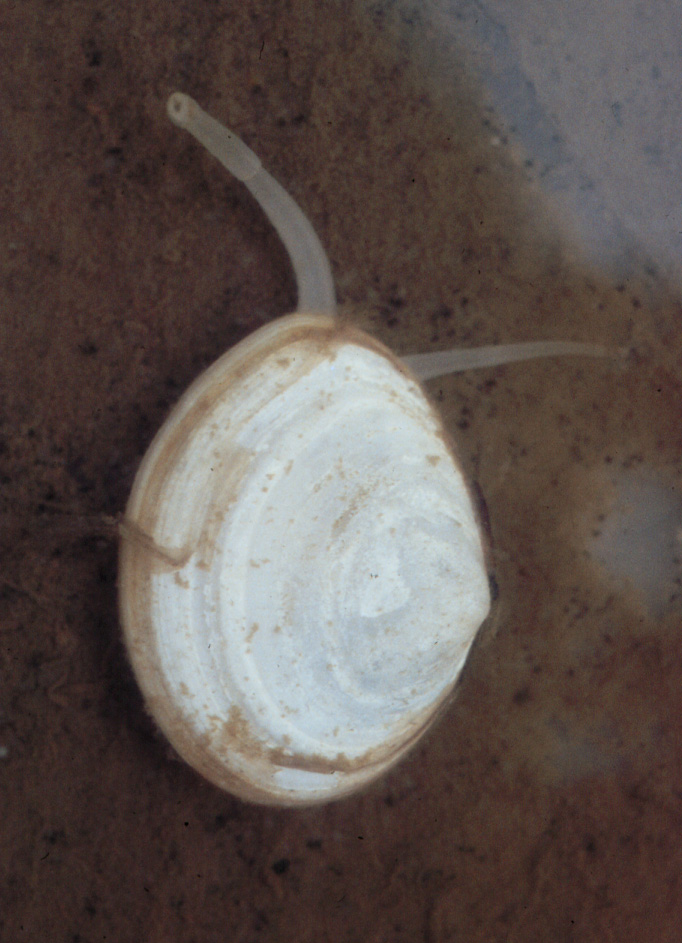
\includegraphics{Macoma_balthica.jpg}
 \end{center}
 
 \end{frame}

\section*{Материал и методика}

\begin{frame}{Районы исследования}
\begin{center}
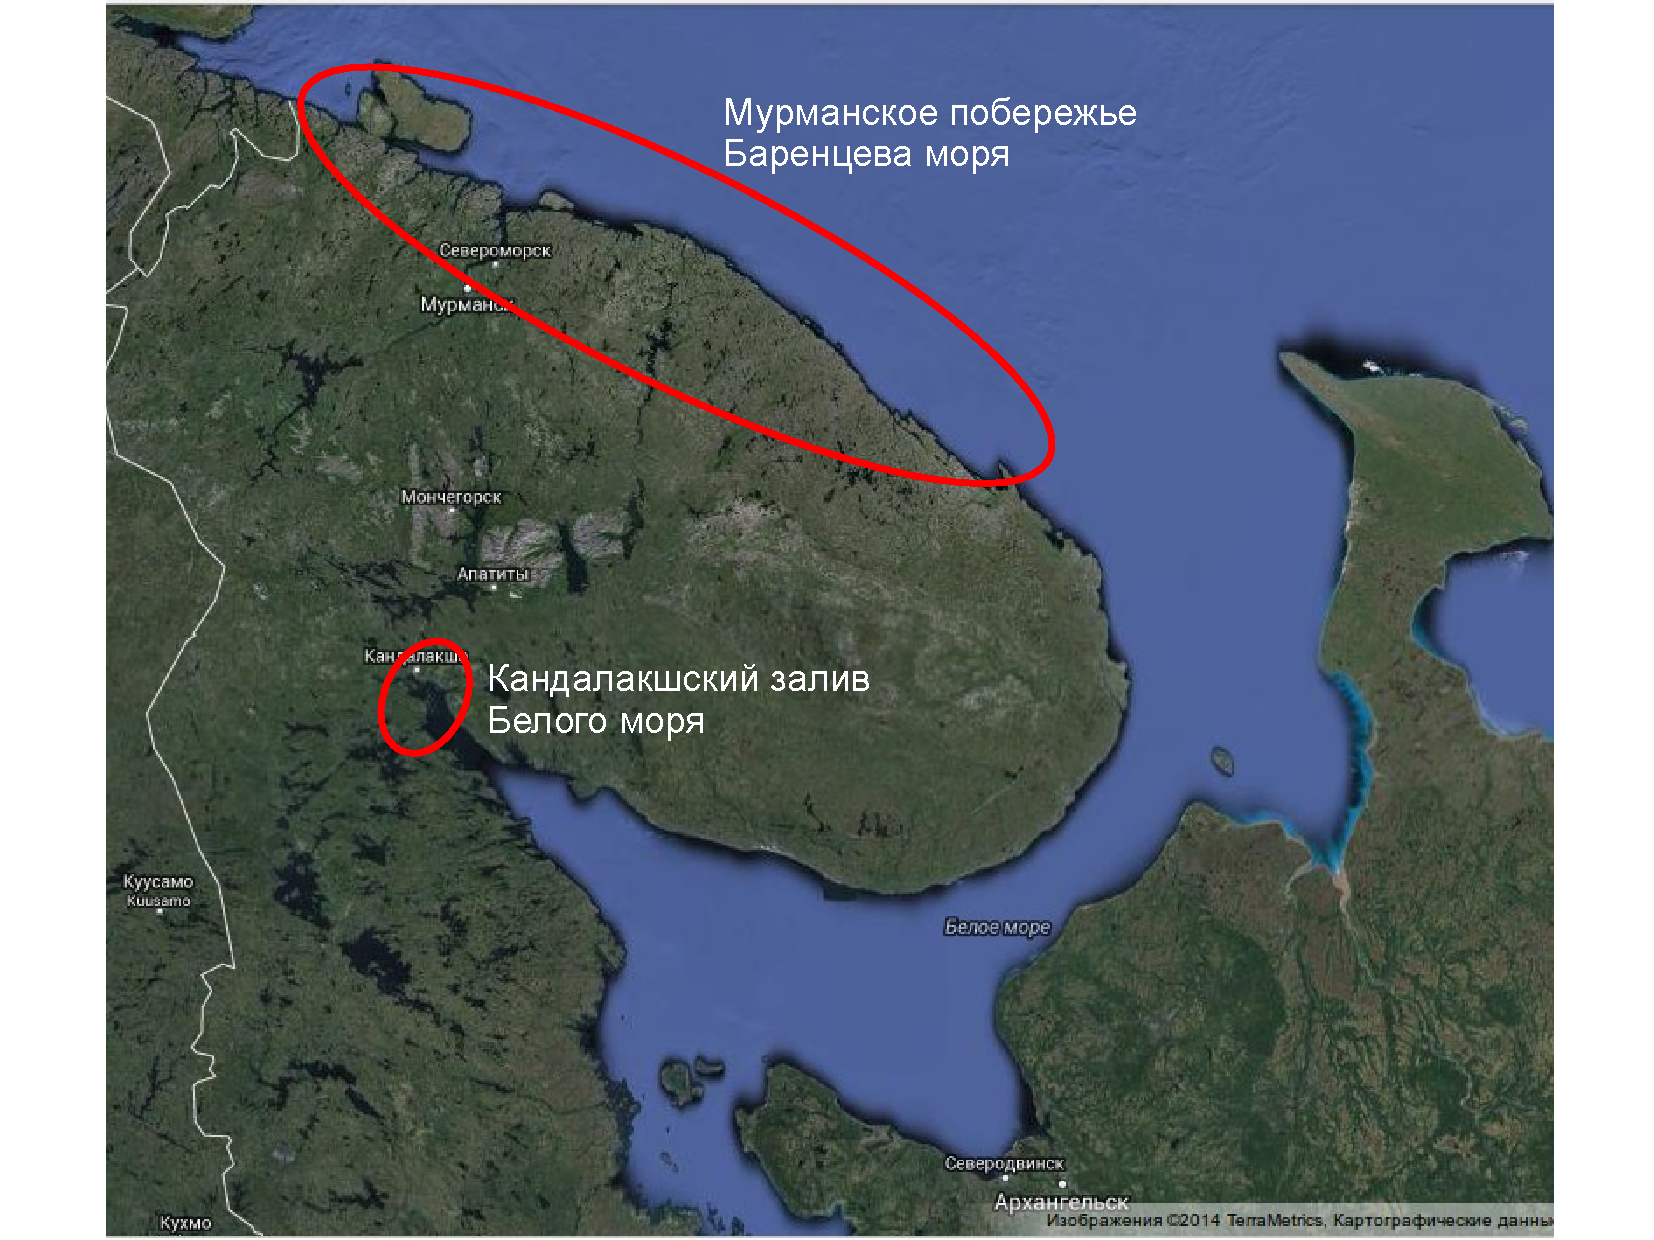
\includegraphics[width=100mm]{./northwest.pdf}

\tiny{maps.google.com}
\end{center}
\end{frame}


\begin{frame}{Исследованные участки: Мурманское побережье Баренцева моря}
\begin{center}
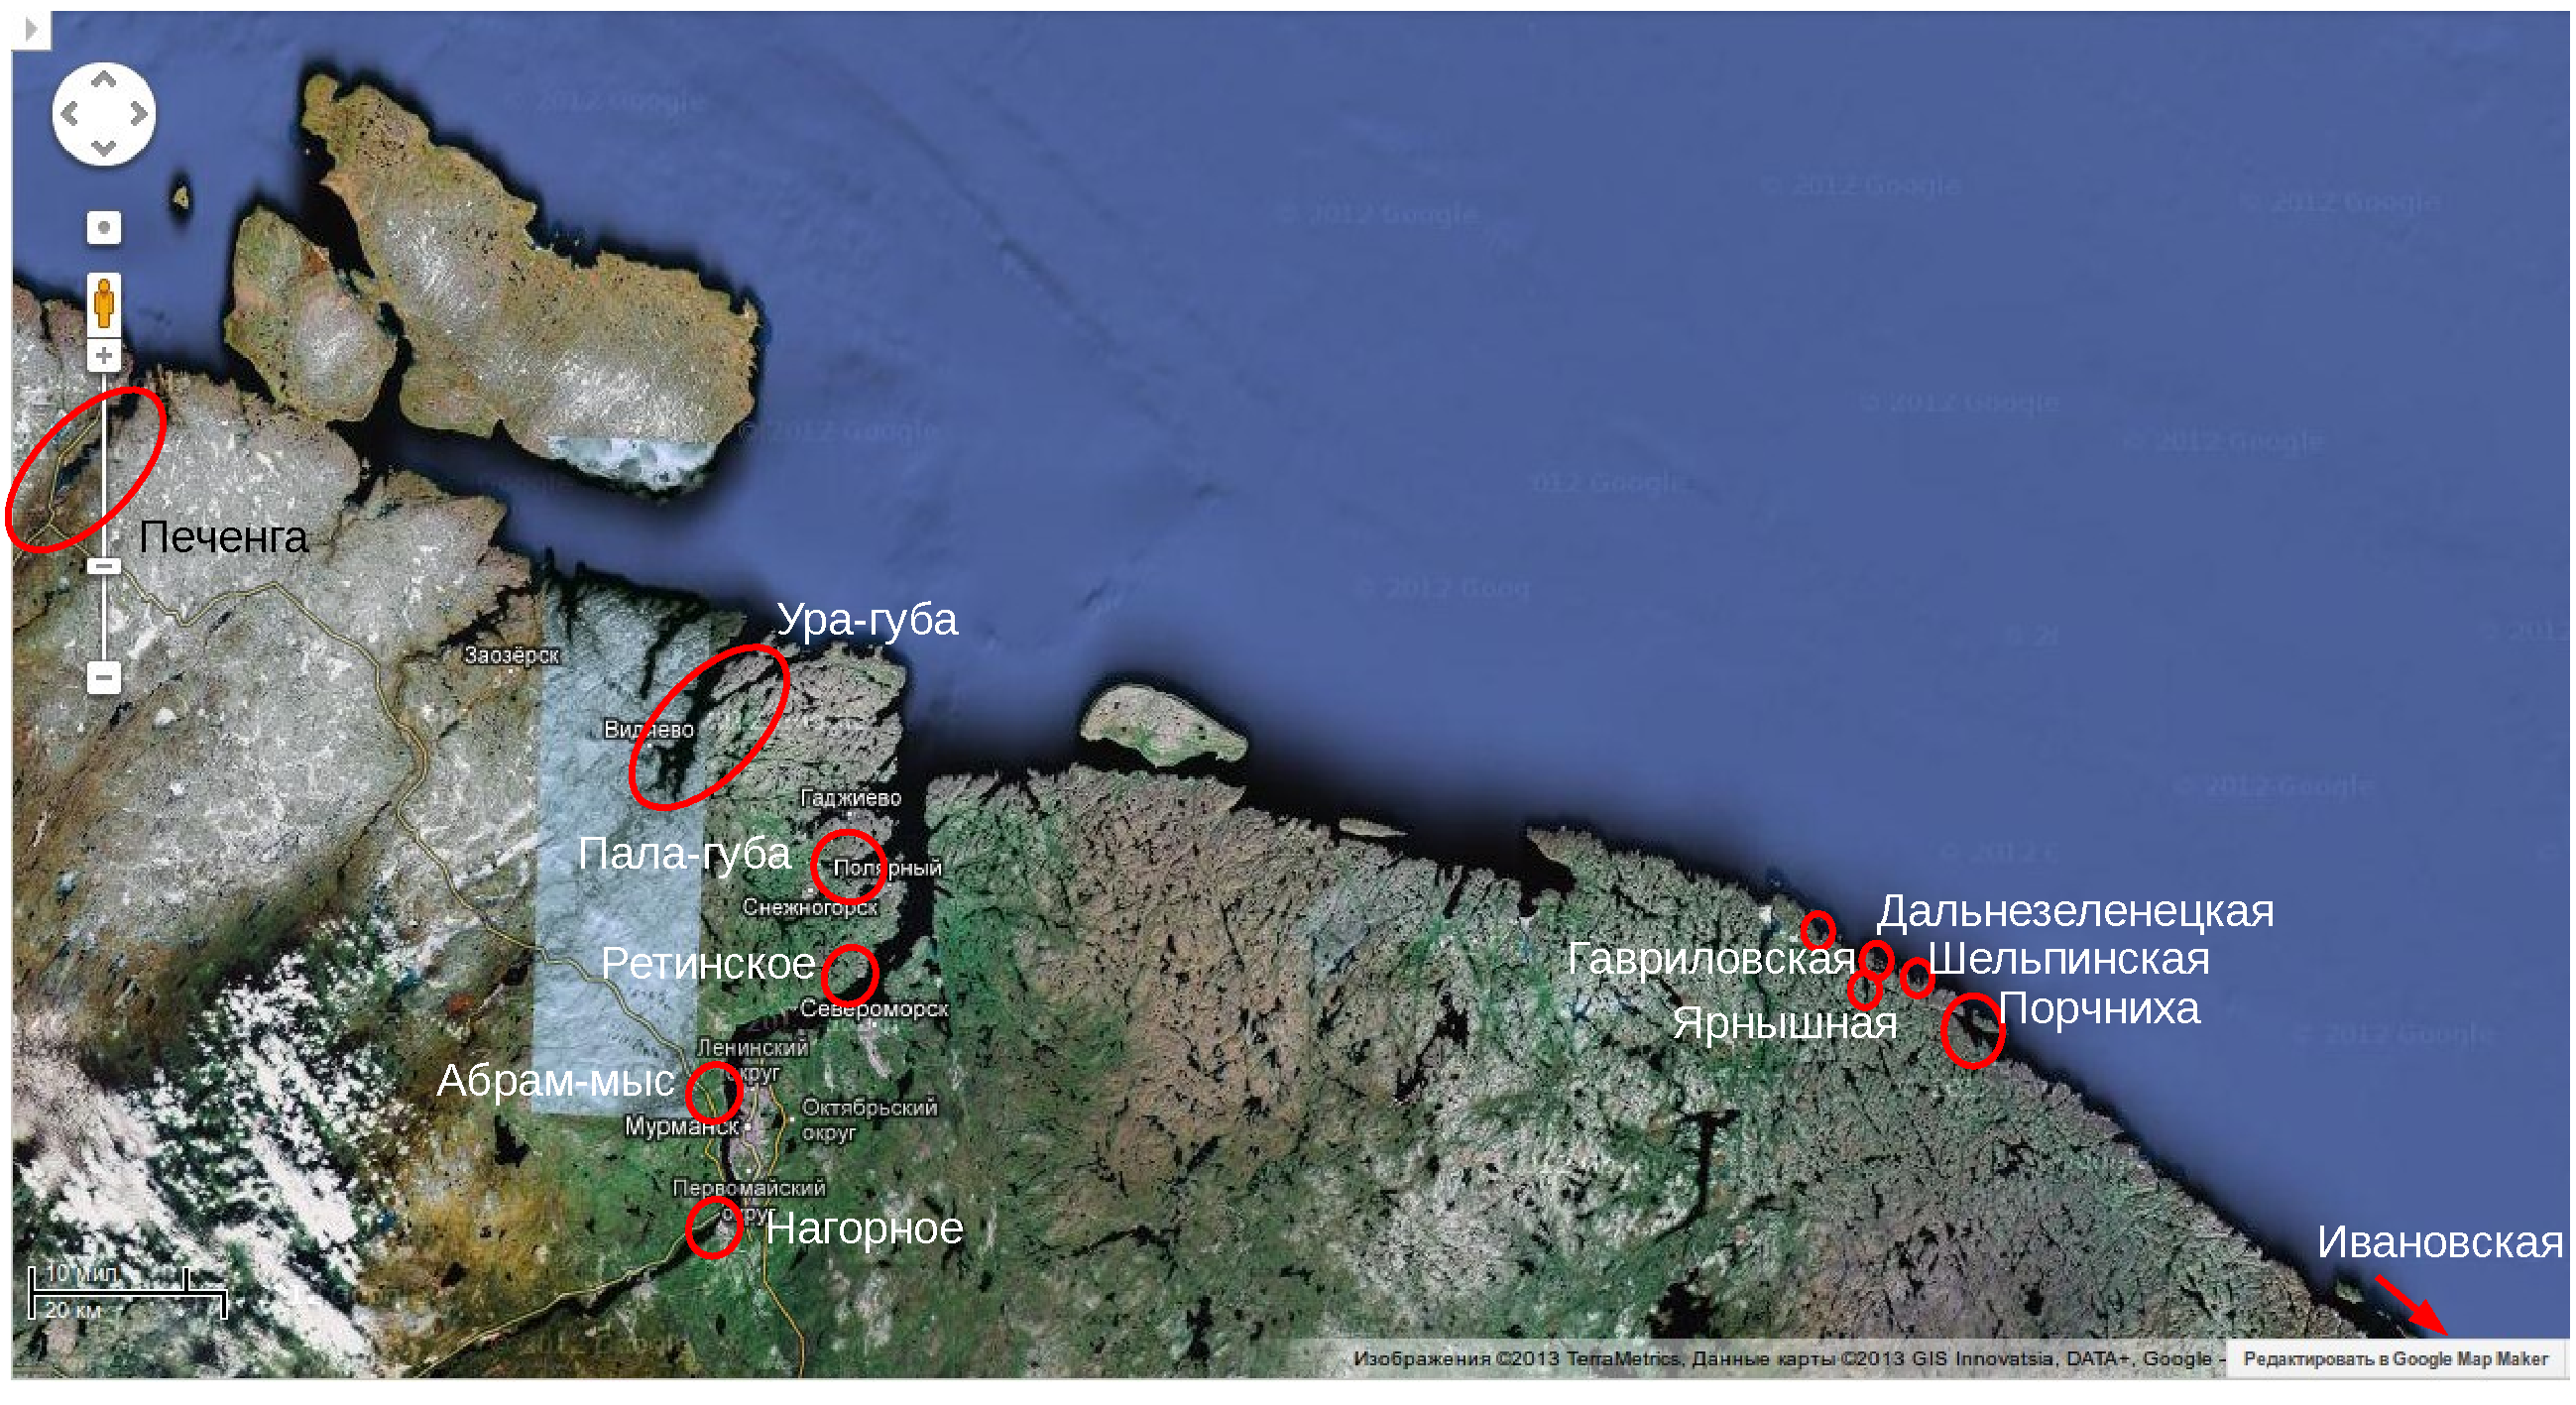
\includegraphics[width=100mm]{./Murman.pdf}

\tiny{maps.google.com}
\end{center}
\end{frame}


\begin{frame}{Кандалакшский залив Белого моря}
\begin{center}
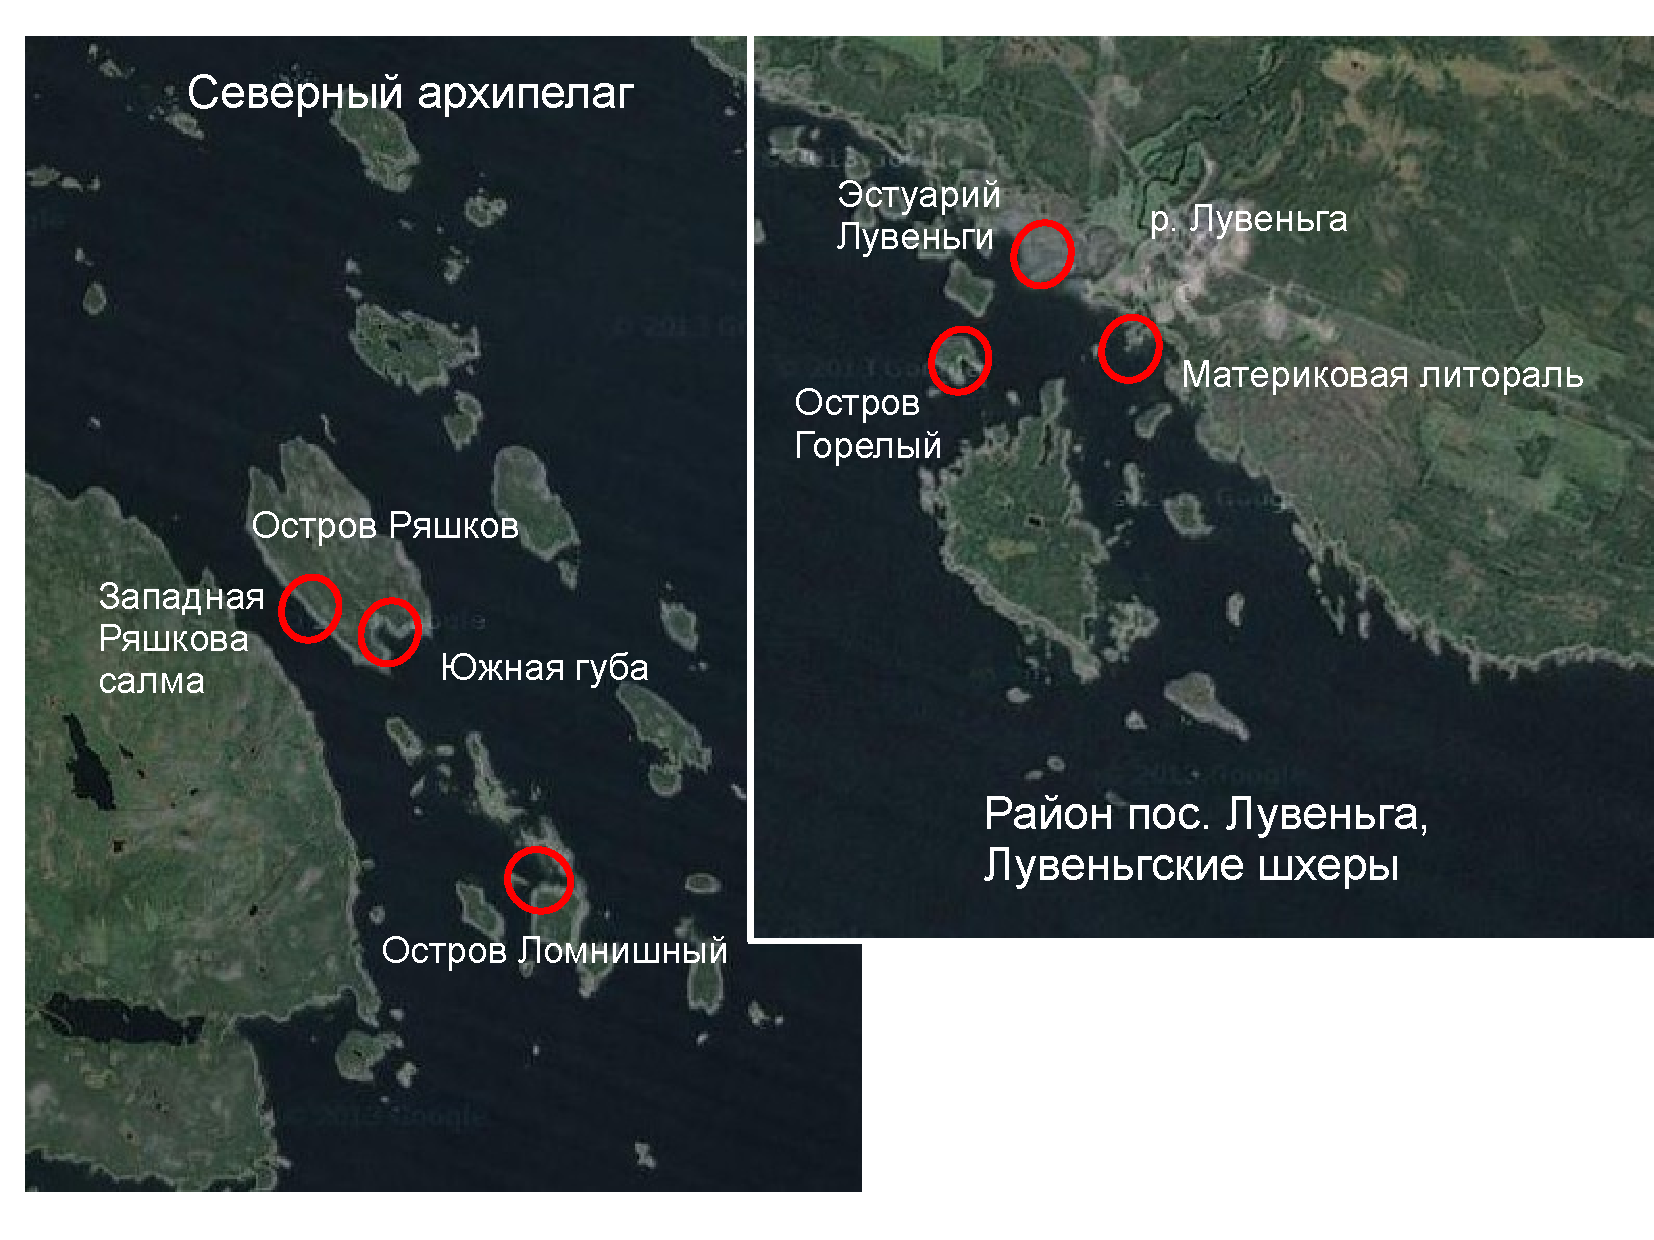
\includegraphics[width=100mm]{./white.pdf}

\tiny{maps.google.com}
\end{center}
\end{frame}

%\begin{frame}{Высказывания о коне}
%\pause
%\begin{block}<+->{Дарт Херохито}
% "Так вот ты какой, северный олень!"
%\end{block}  \pause

%\begin{block}{Кавалерия Новодворская}
% "Сферический конь борозды не портит"
%\end{block} \pause

%\begin{block}{Русская женщина}
% "Да я его на скаку!"
%\end{block} 
%\end{frame}




	\section{Пространственное распределение {\it Macoma~balthica}}
\begin{frame}{Вертикальное распределение {\it Macoma~balthica} на литорали}
% barplot по нашим участкам
\begin{figure}
\begin{minipage}[b]{.3\linewidth}
	\begin{center}
\tiny{о.~Горелый}
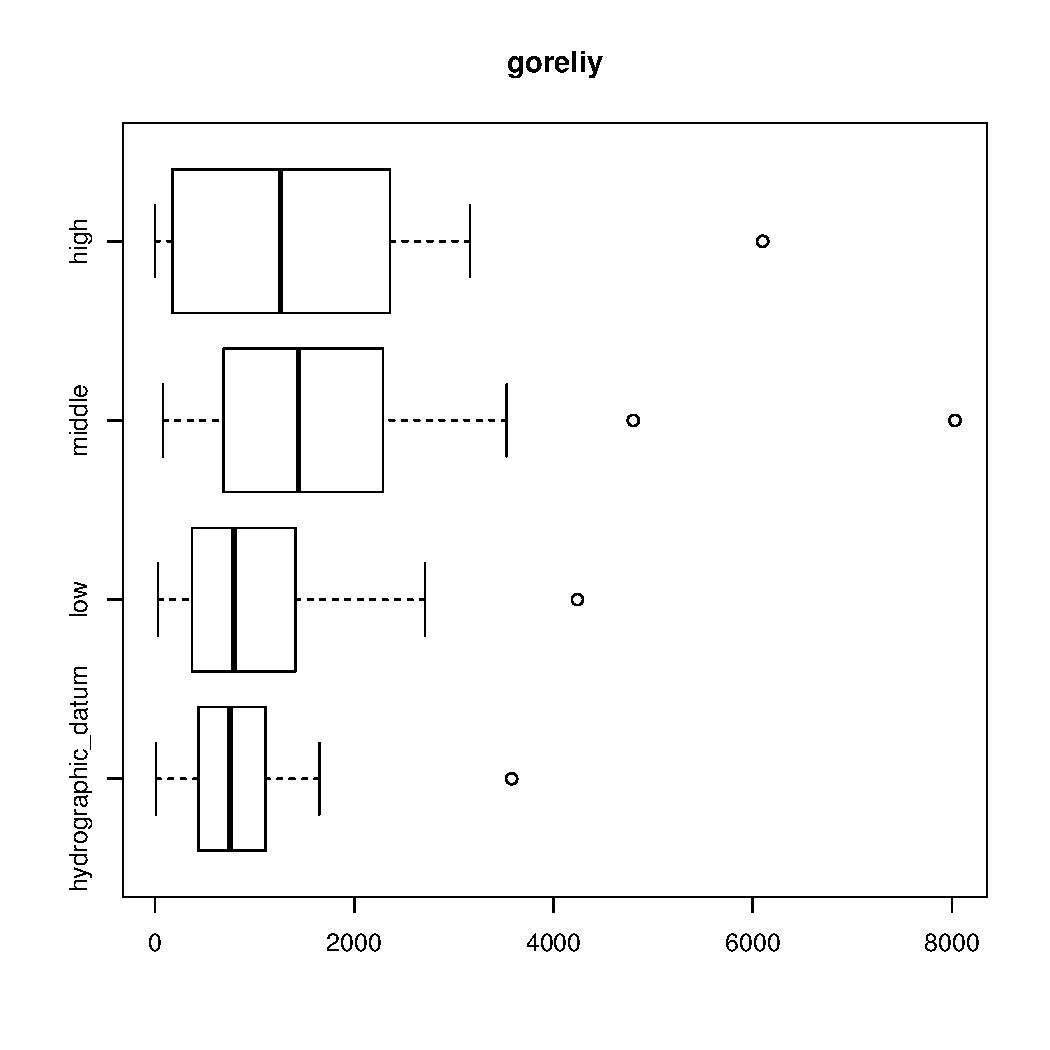
\includegraphics[width=33mm]{./Vertikal_strukture/goreliy_vertical.pdf}
	\end{center}
	\end{minipage}
	\hfil %Это пружинка отодвигающая рисунки друг от друга
	\begin{minipage}[b]{.3\linewidth}
	\begin{center}
\tiny{Пала-губа}
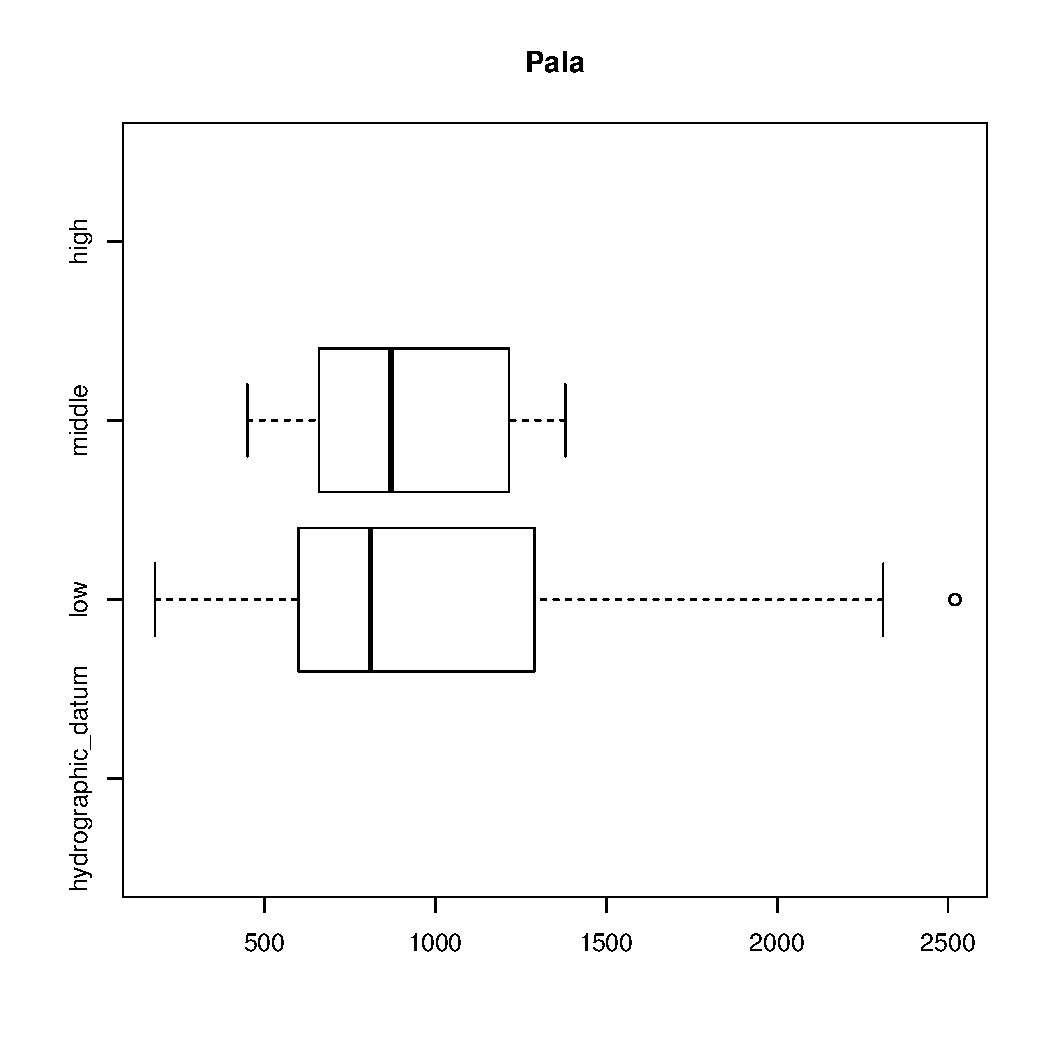
\includegraphics[width=33mm]{./Vertikal_strukture/Pala_vertical.pdf}
	\end{center}
	\end{minipage}
	\hfil %Это пружинка отодвигающая рисунки друг от друга
	\begin{minipage}[b]{.3\linewidth}
	\begin{center}
\tiny{Дальнезеленецкая}
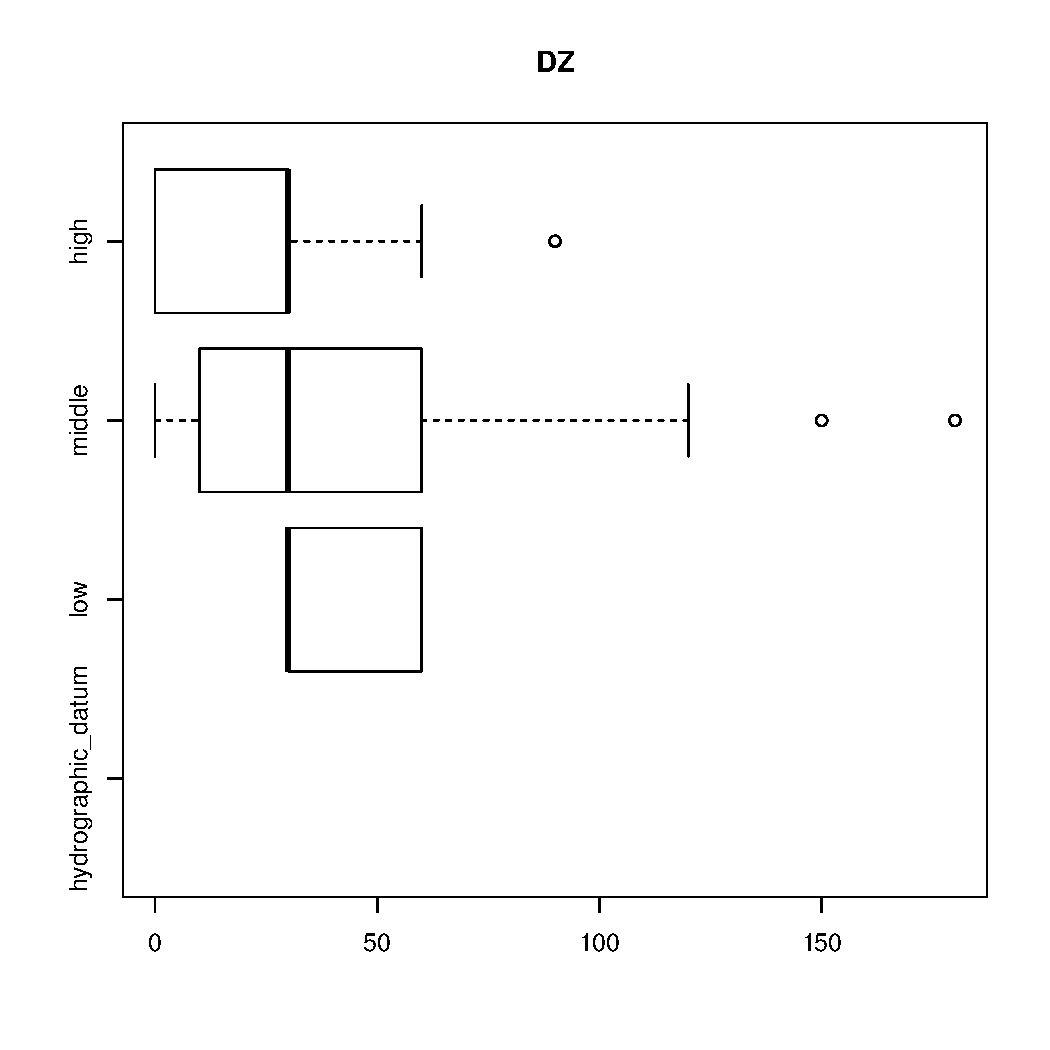
\includegraphics[width=33mm]{./Vertikal_strukture/DZ_vertical.pdf}
	\end{center}
	\end{minipage}
	\begin{minipage}[b]{.3\linewidth}
	\begin{center}
\tiny{материк, Лувеньга}
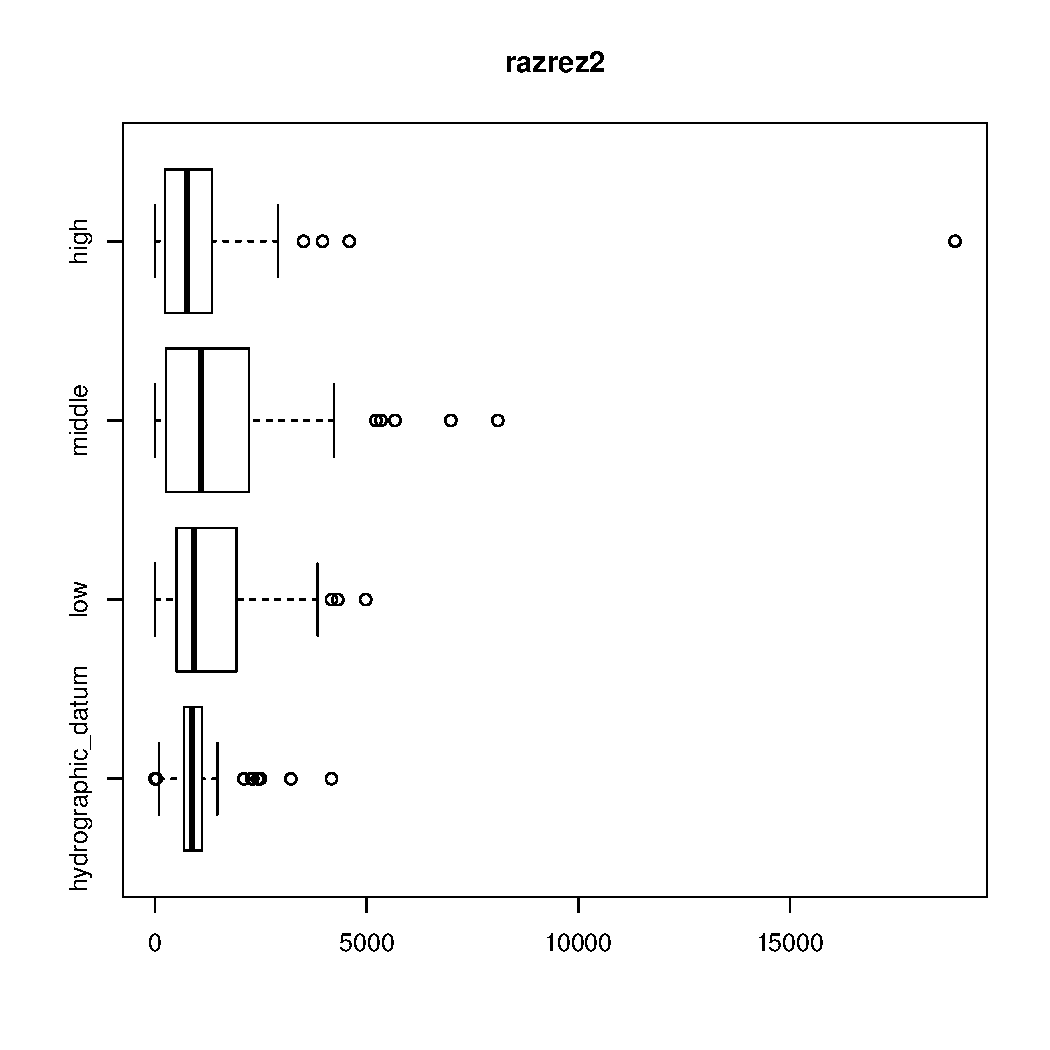
\includegraphics[width=33mm]{./Vertikal_strukture/razrez2_vertical.pdf}
	\end{center}
	\end{minipage}
	\hfil %Это пружинка отодвигающая рисунки друг от друга
	\begin{minipage}[b]{.3\linewidth}
	\begin{center}
\tiny{Абрам-мыс}
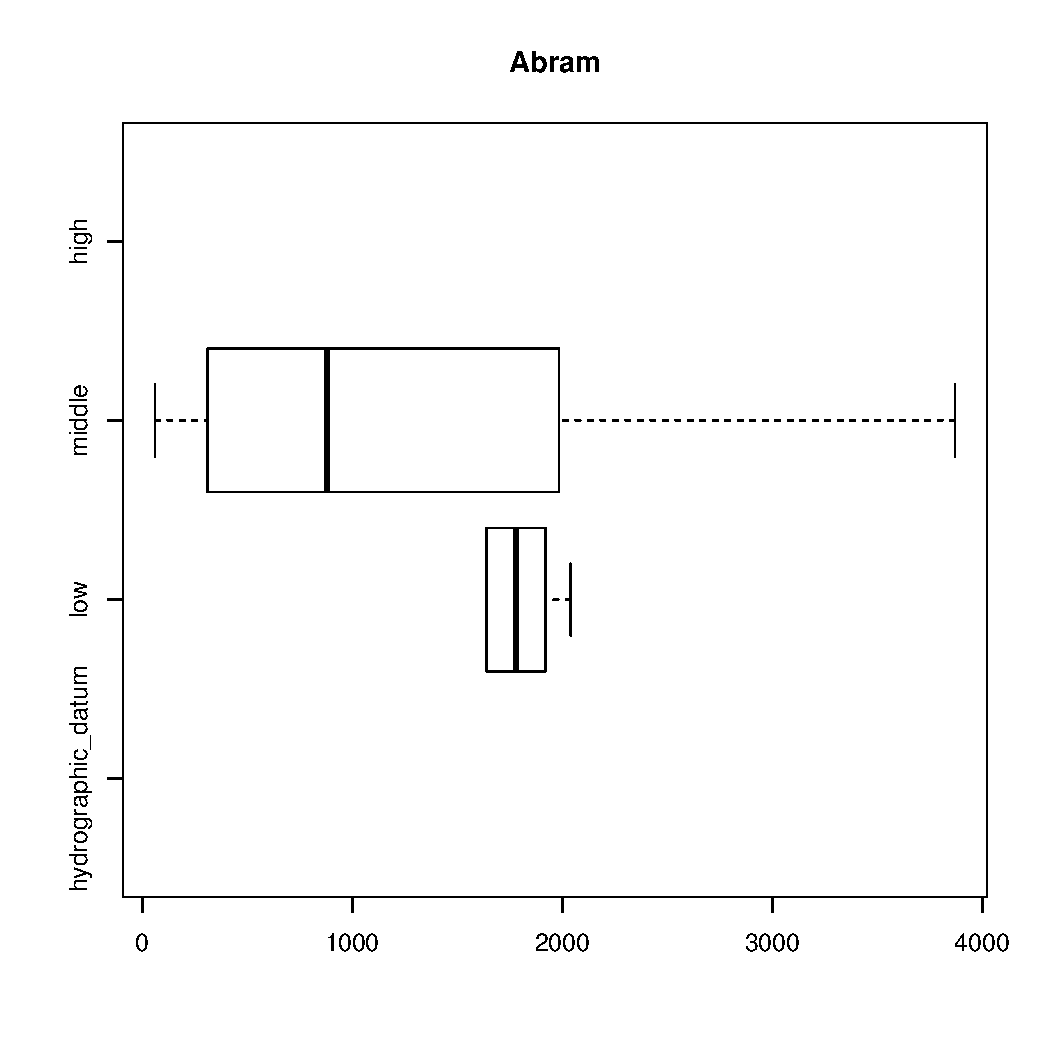
\includegraphics[width=33mm]{./Vertikal_strukture/Abram_vertical.pdf}
	\end{center}
	\end{minipage}
	\hfil %Это пружинка отодвигающая рисунки друг от друга
	\begin{minipage}[b]{.3\linewidth}
	\begin{center}
\tiny{Ярнышная}
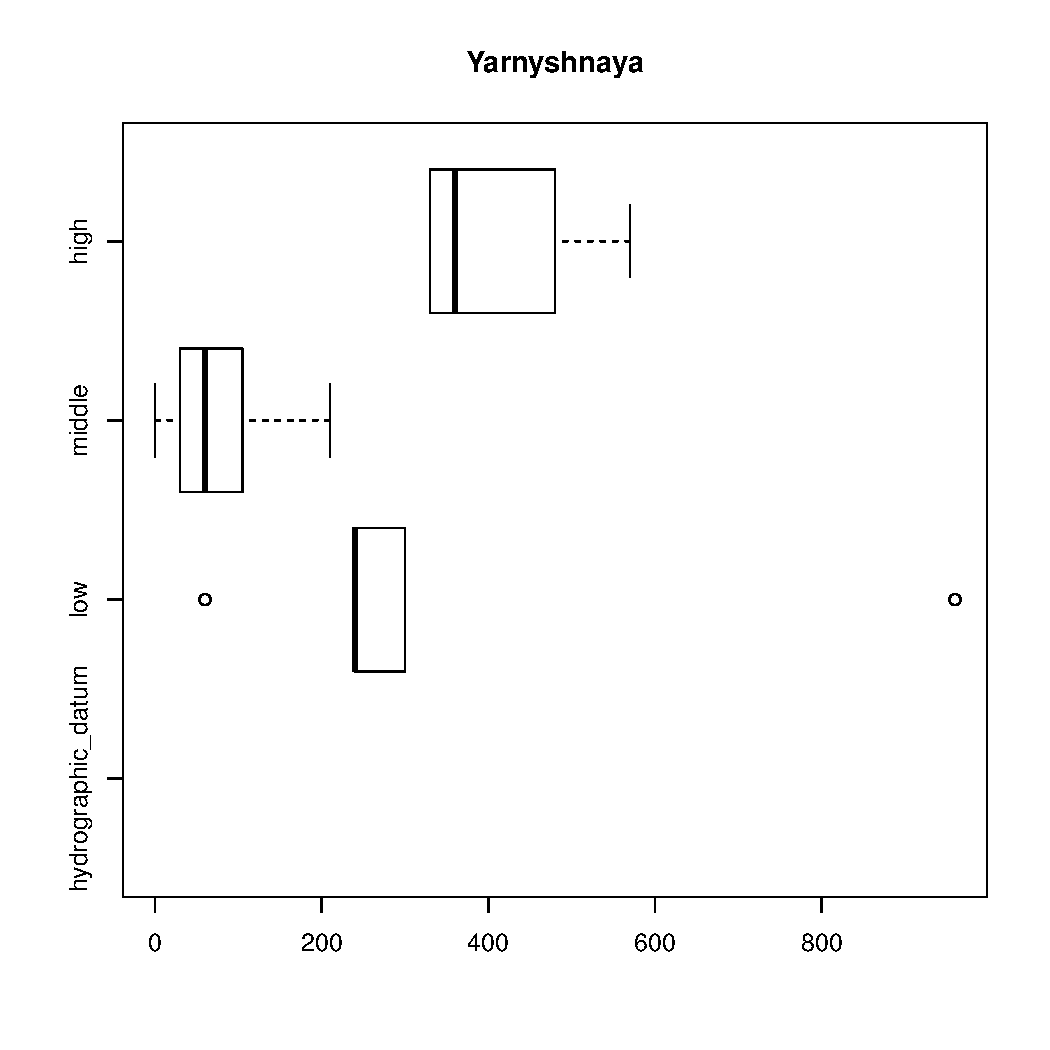
\includegraphics[width=33mm]{./Vertikal_strukture/Yarnyshnaya_vertical.pdf}
	\end{center}
	\end{minipage}
\end{figure}
\end{frame}

%\begin{frame}{существуют ли <<Детские сады>> (nurseries)?}
% barplot по нашим участкам

%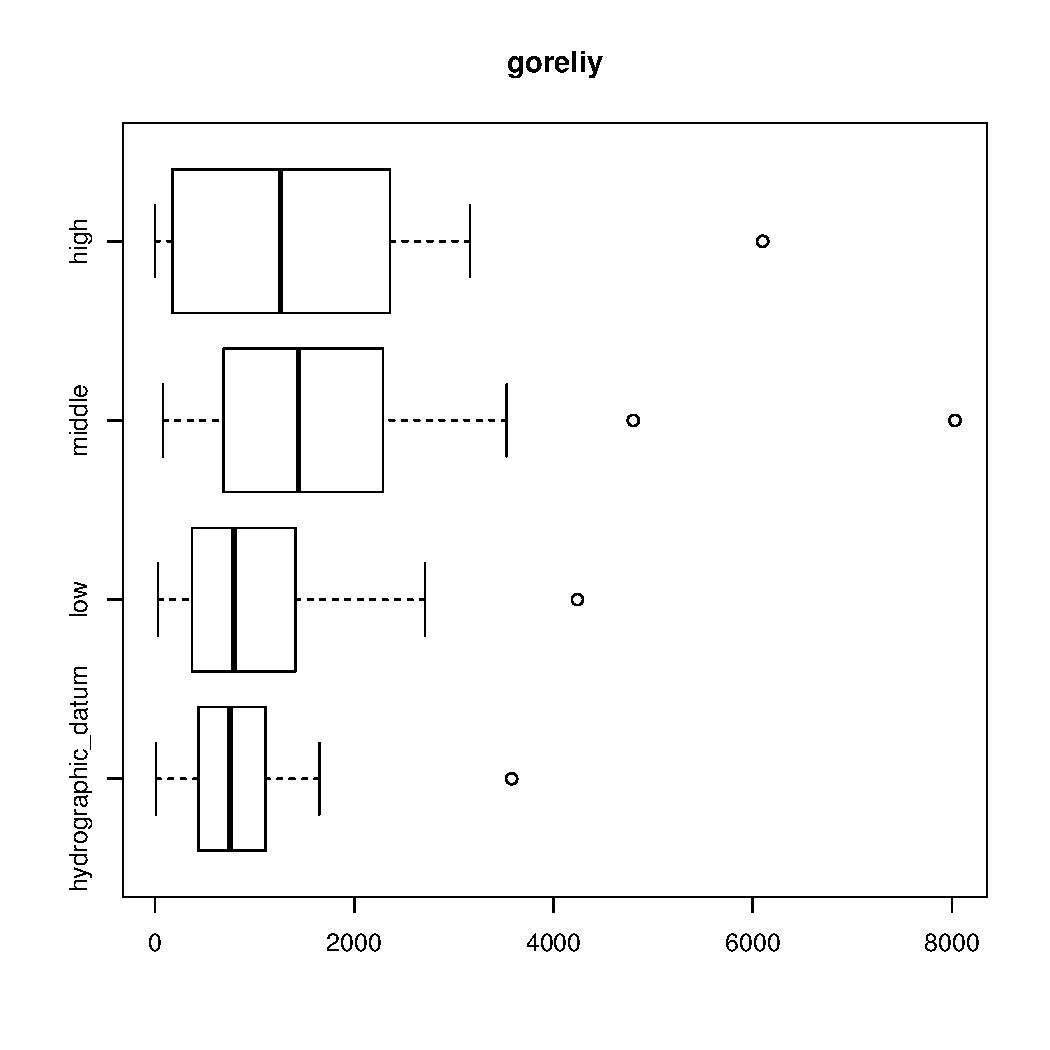
\includegraphics[width=100pt, height=100pt]{./Vertikal_strukture/goreliy_vertical.pdf}

%\end{frame}
	

\begin{frame}{Микрораспределение {\it Macoma~balthica}}
\framesubtitle{Схема пробоотбора (масштабирование методики из Trush et al, 1989)}
\tiny{Полигон $7,5 \times 12$~м. $12$ квадратов, по $3$ случайно взятых пробы с фиксацией координат. Всего $36$ проб.}
\begin{figure}
	\begin{minipage}[b]{.49\linewidth}
	\begin{center}
\tiny{Дальнезеленецкая, 2007}
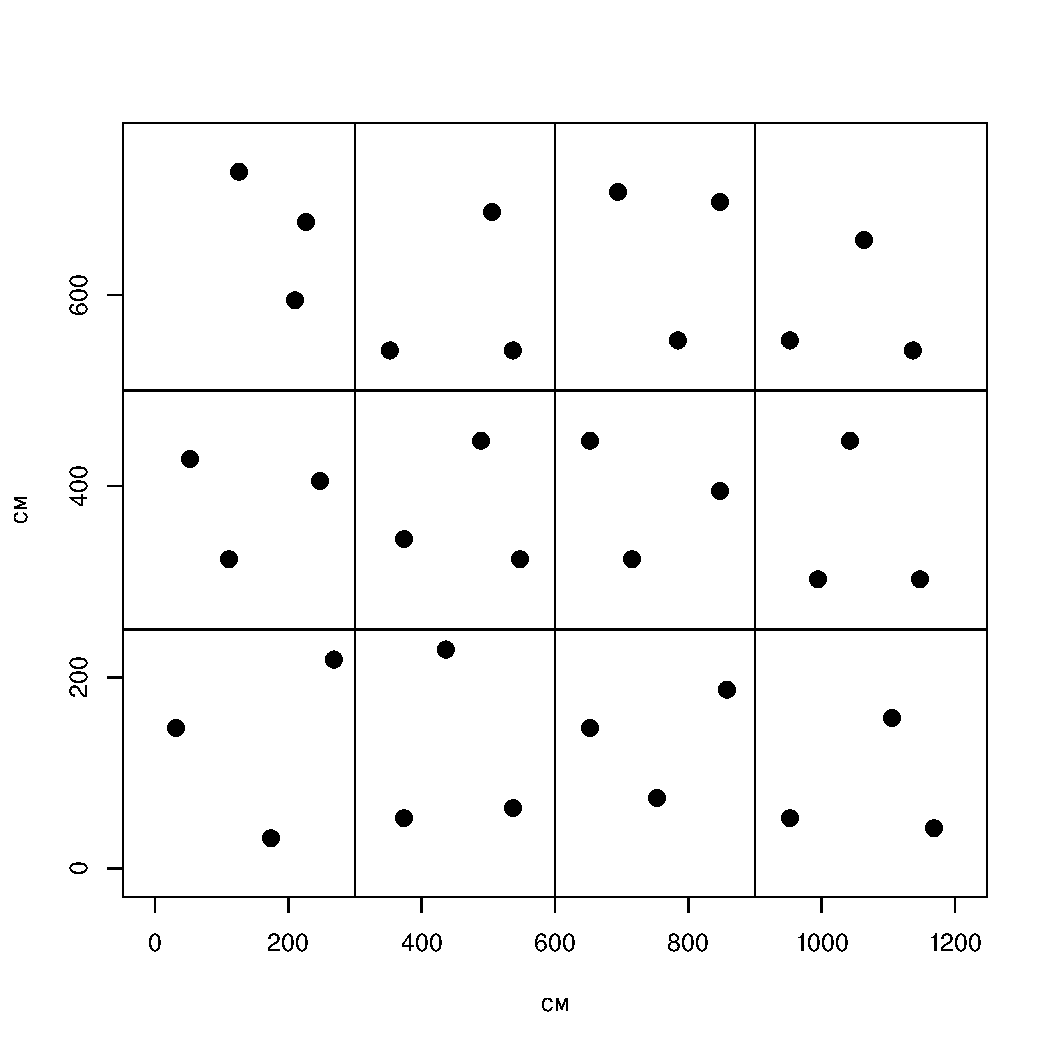
\includegraphics[width=35mm]{./microdistribution/Plyazh07_samples.pdf}
	\end{center}
	\end{minipage}
\hfil %Это пружинка отодвигающая рисунки друг от друга
	\begin{minipage}[b]{.49\linewidth}
\begin{center}
\tiny{Дальнезеленецкая, 2008. 2 полигона}
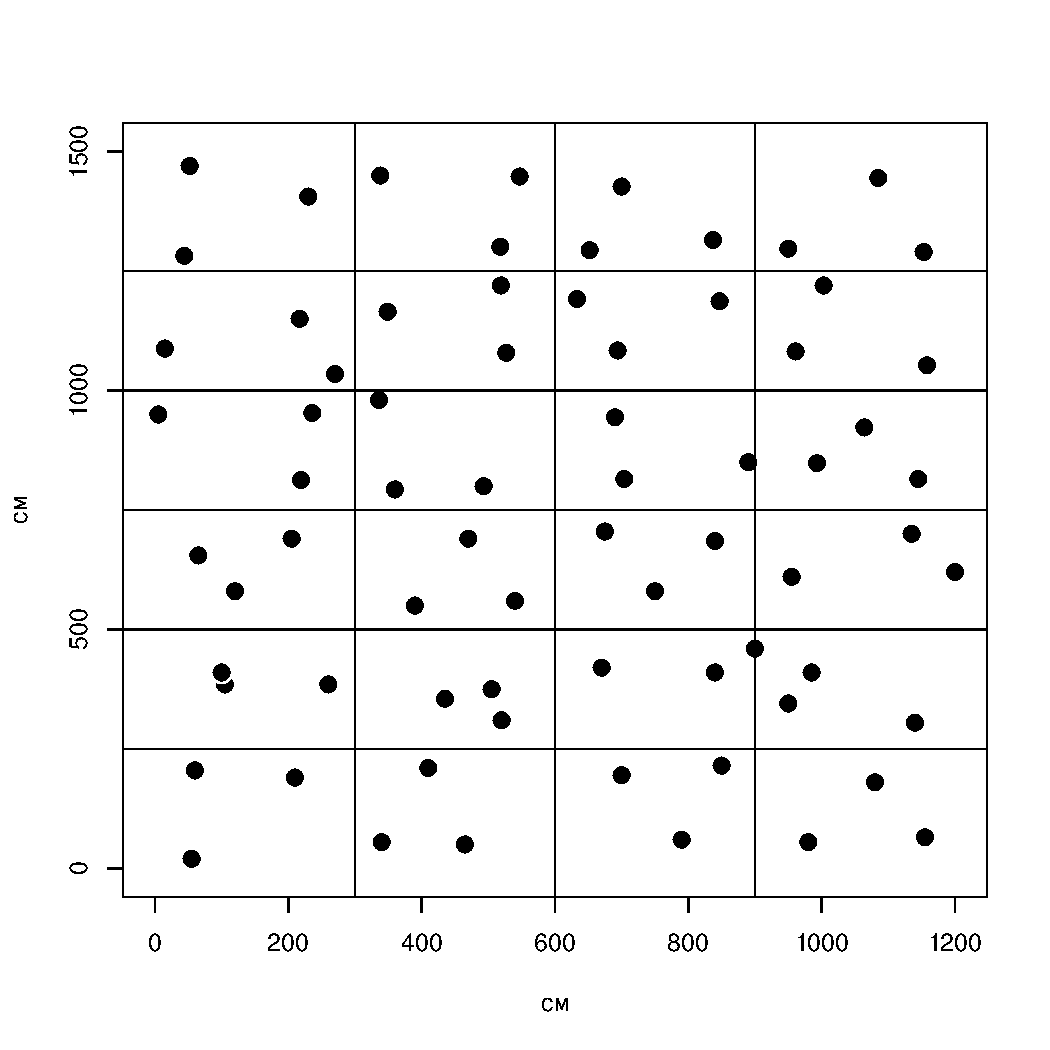
\includegraphics[width=35mm]{./microdistribution/Plyazh08_samples.pdf}
	\end{center}
	\end{minipage}
	\begin{minipage}[b]{.49\linewidth}
	\begin{center}
\tiny{Ярнышная, 2008}
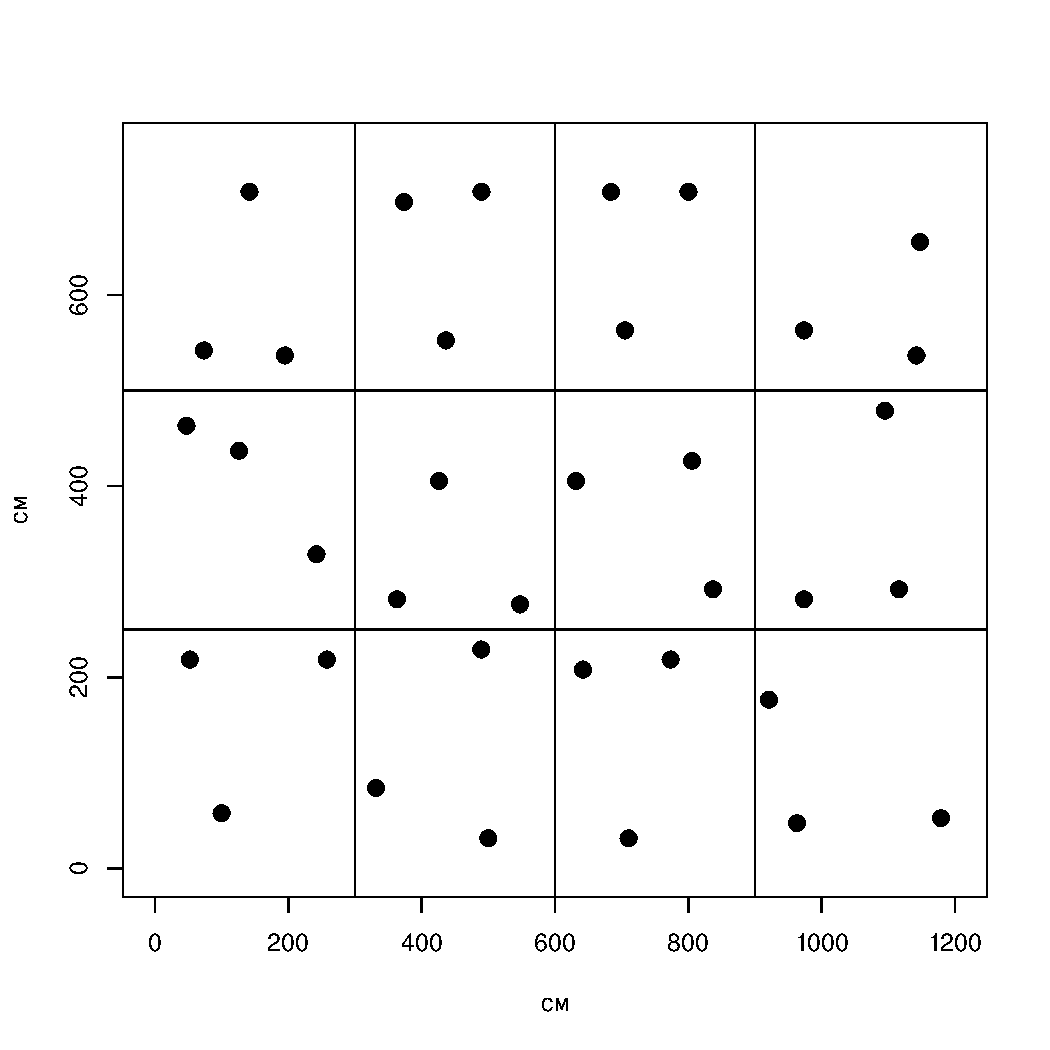
\includegraphics[width=35mm]{./microdistribution/Yarnyshnaya_samples.pdf}
	\end{center}
	\end{minipage}
\hfil %Это пружинка отодвигающая рисунки друг от друга
	\begin{minipage}[b]{.49\linewidth}
	\begin{center}
\tiny{Пала-губа, 2008}
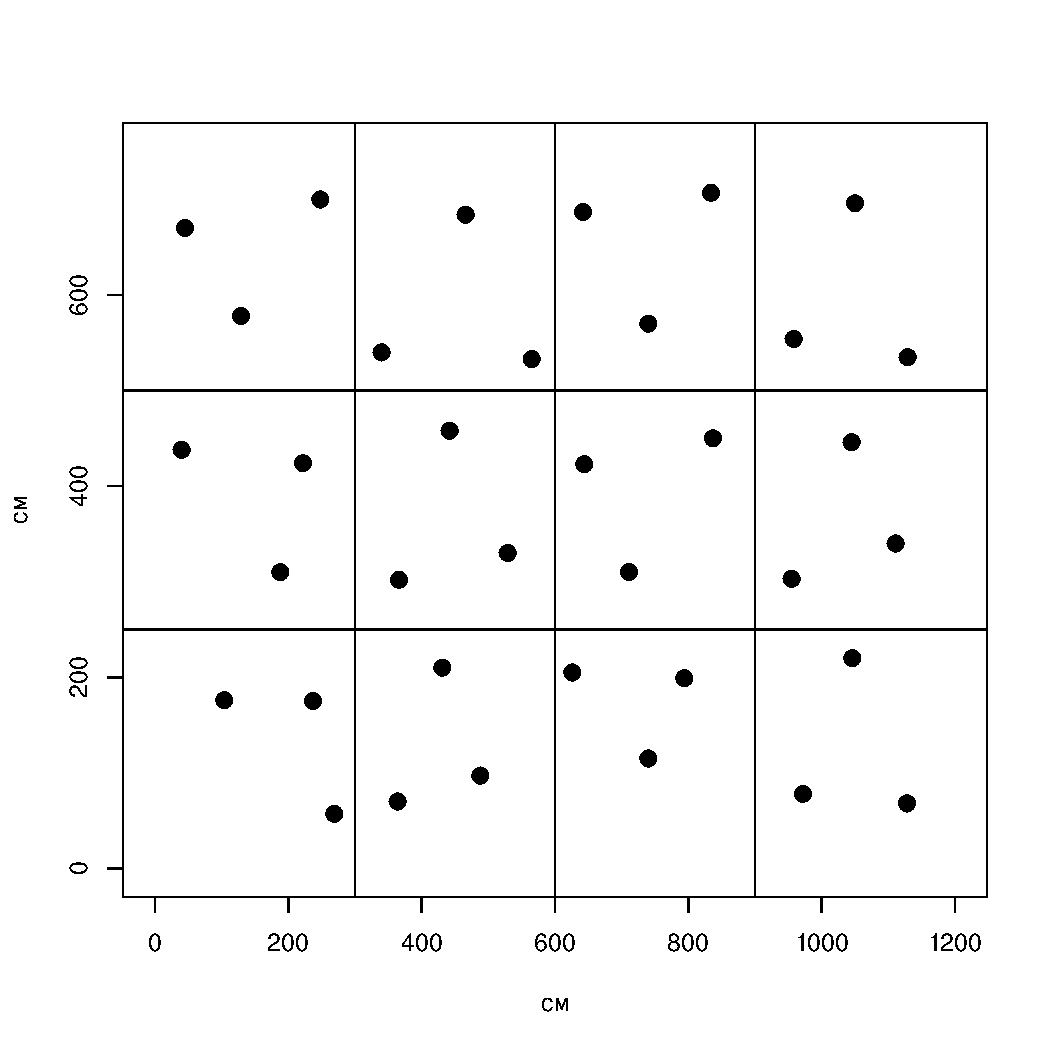
\includegraphics[width=35mm]{./microdistribution/Pala_samples.pdf}
	\end{center}
	\end{minipage}
\end{figure}
\end{frame}

\begin{frame}{Микрораспределение {\it Macoma~balthica}}
\framesubtitle{Дальний пляж губы Дальнезеленецкая}
% микрораспределение по обилию
\begin{figure}
	\begin{minipage}[b]{.49\linewidth}
\tiny{Дальнезеленецкая, 2007}
	\begin{center}
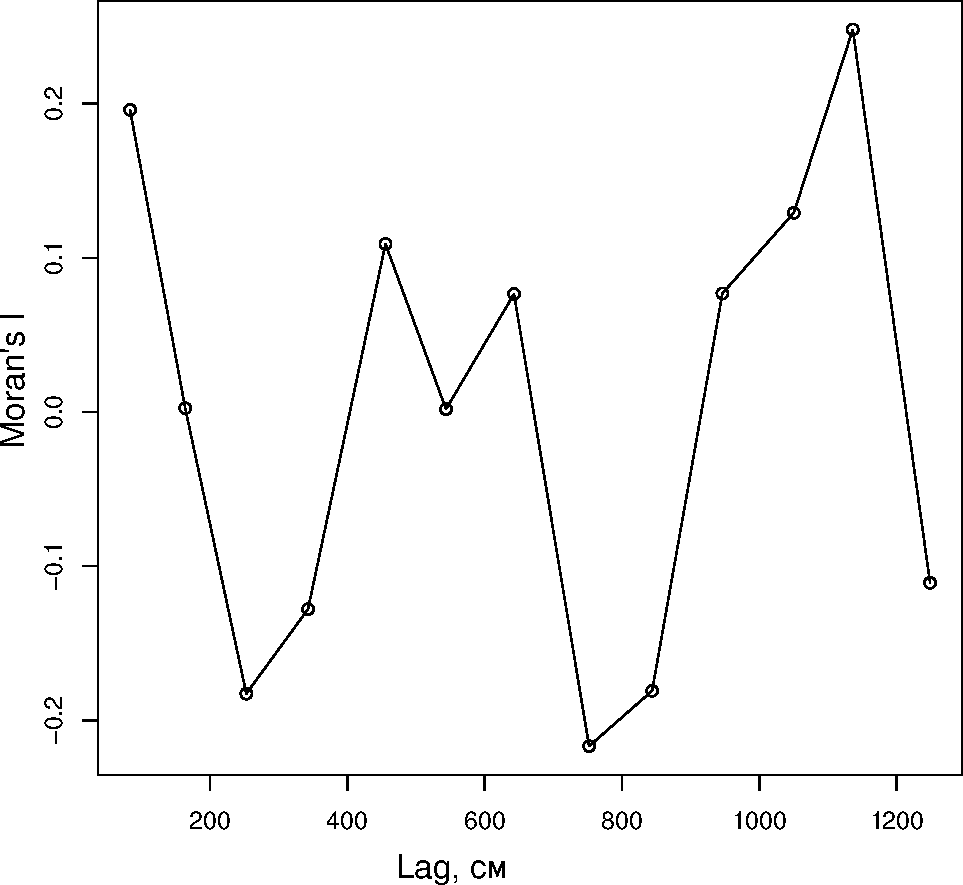
\includegraphics[width=35mm]{./microdistribution/Plyazh07_moran_N_Macoma_balthica_.pdf}
	\end{center}
	\end{minipage}
\hfil %Это пружинка отодвигающая рисунки друг от друга
	\begin{minipage}[b]{.49\linewidth}
	\begin{center}
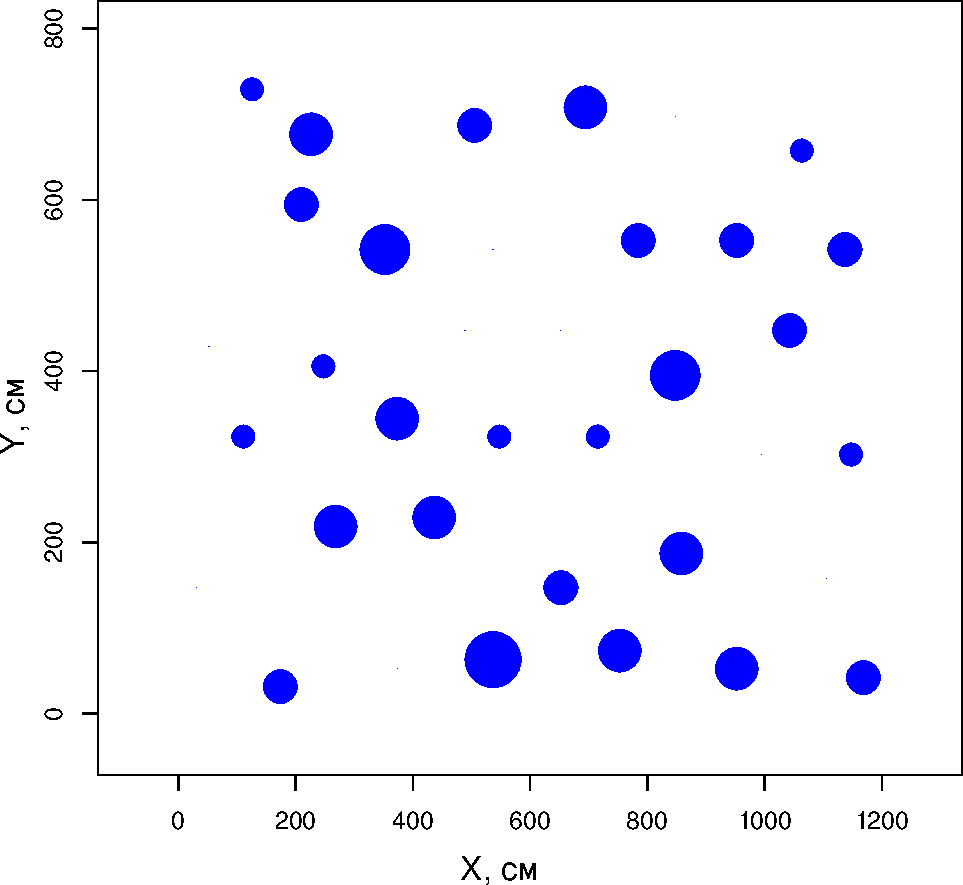
\includegraphics[width=35mm]{./microdistribution/Plyazh07_N_Macoma_bubbles.pdf}
	\end{center}
	\end{minipage}
	\begin{minipage}[b]{.49\linewidth}
\tiny{Дальнезеленецкая, 2008}
	\begin{center}
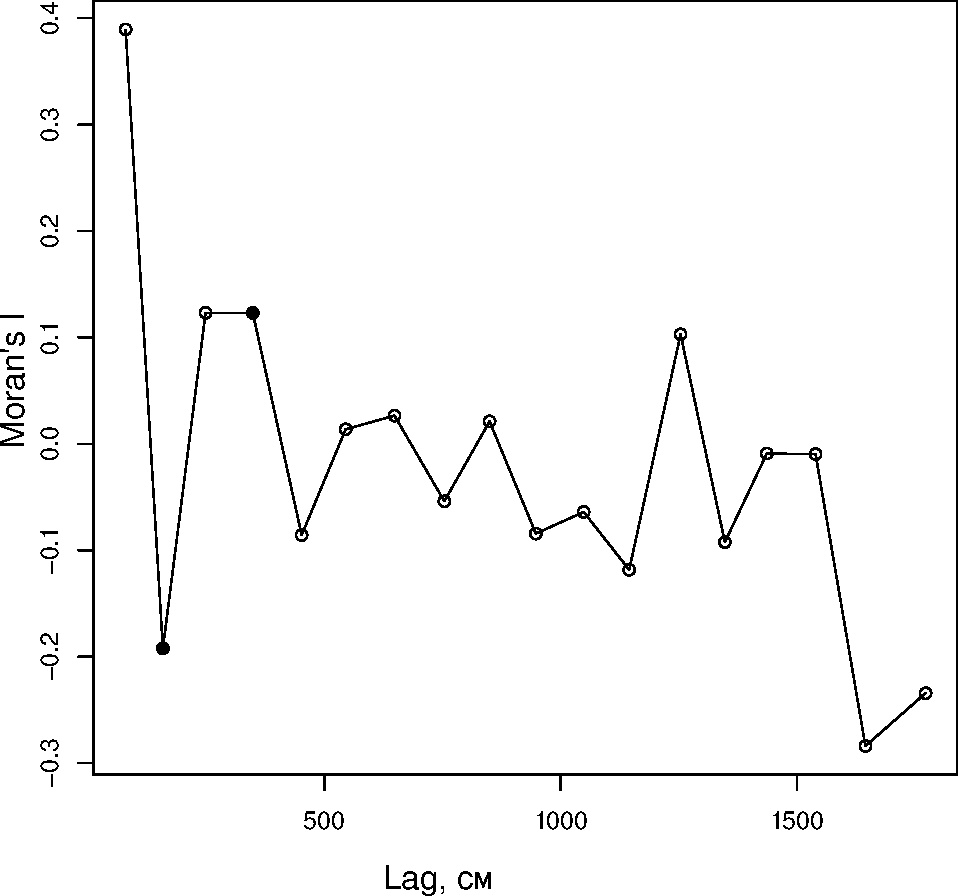
\includegraphics[width=35mm]{./microdistribution/Plyazh0812_moran_N_Macoma_balthica_.pdf}
	\end{center}
	\end{minipage}
\hfil %Это пружинка отодвигающая рисунки друг от друга
	\begin{minipage}[b]{.49\linewidth}
	\begin{center}
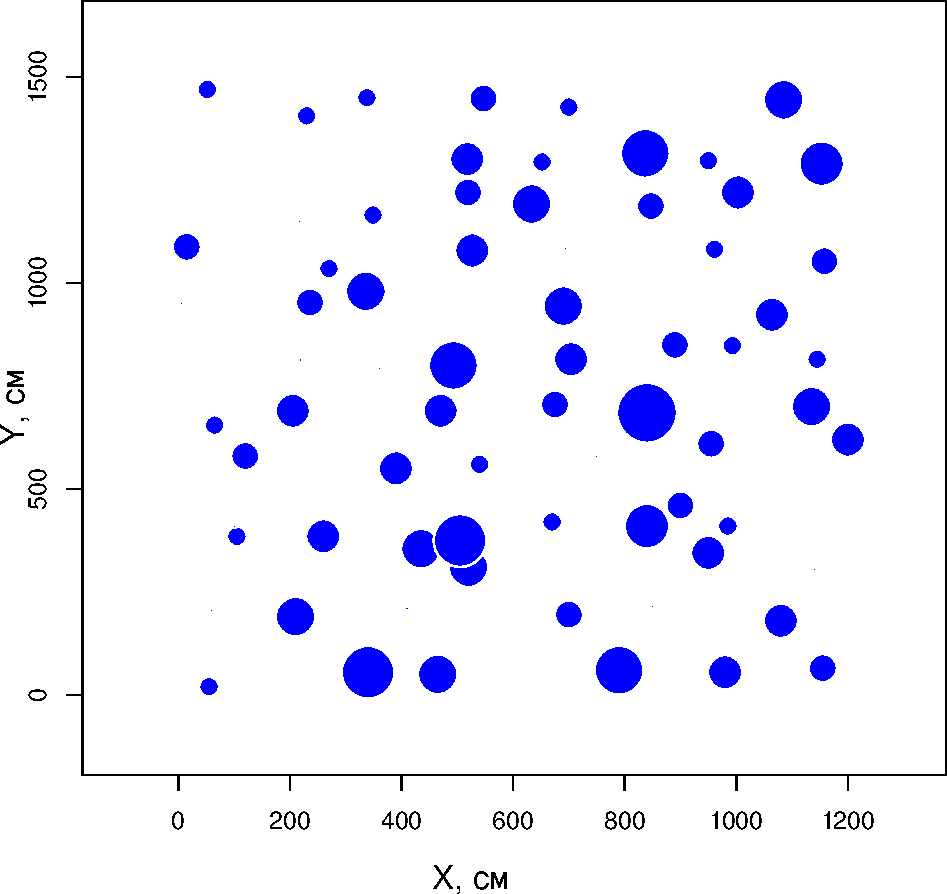
\includegraphics[width=35mm]{./microdistribution/Plyazh0812_N_Macoma_bubbles.pdf}
	\end{center}
	\end{minipage}
\end{figure}
\end{frame}


\begin{frame}{Микрораспределение {\it Macoma~balthica}}
\framesubtitle{бухта Ярнышная}
% микрораспределение по обилию
\begin{figure}
\begin{minipage}[b]{.49\linewidth}
	\begin{center}
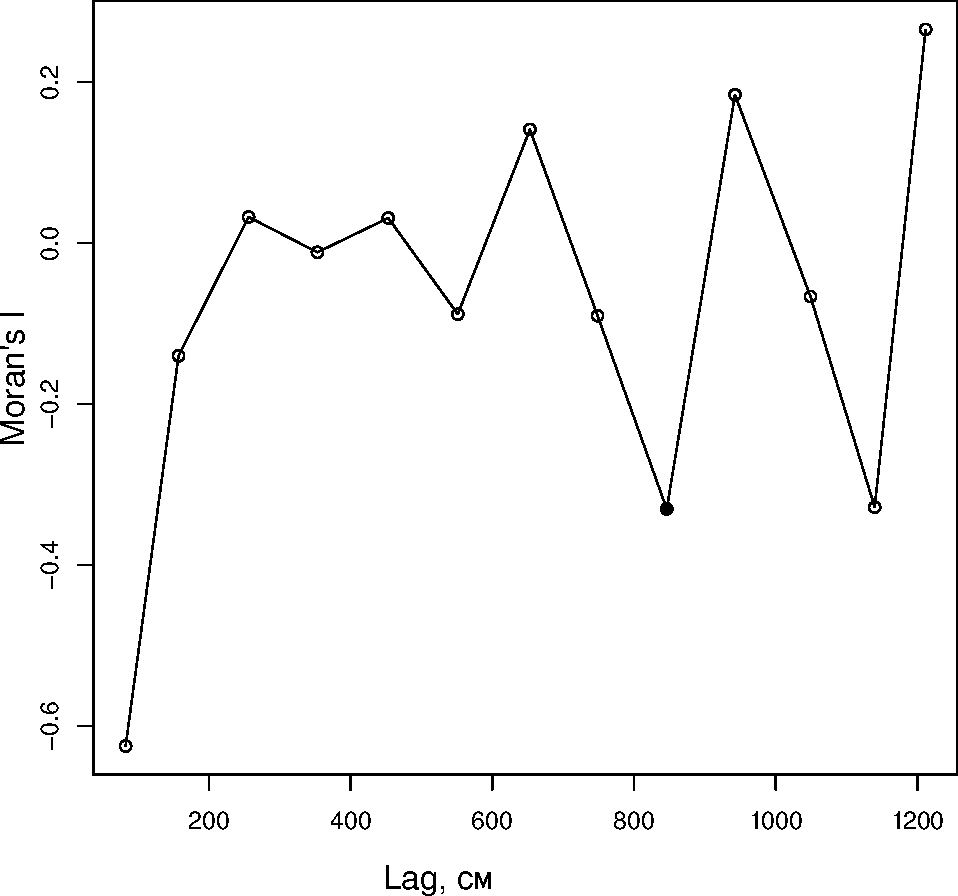
\includegraphics[width=49mm]{./microdistribution/Yarnyshnaya07_moran_N_Macoma_balthica_.pdf}
\end{center}
	\end{minipage}
	\hfil %Это пружинка отодвигающая рисунки друг от друга
	\begin{minipage}[b]{.49\linewidth}
\begin{center}
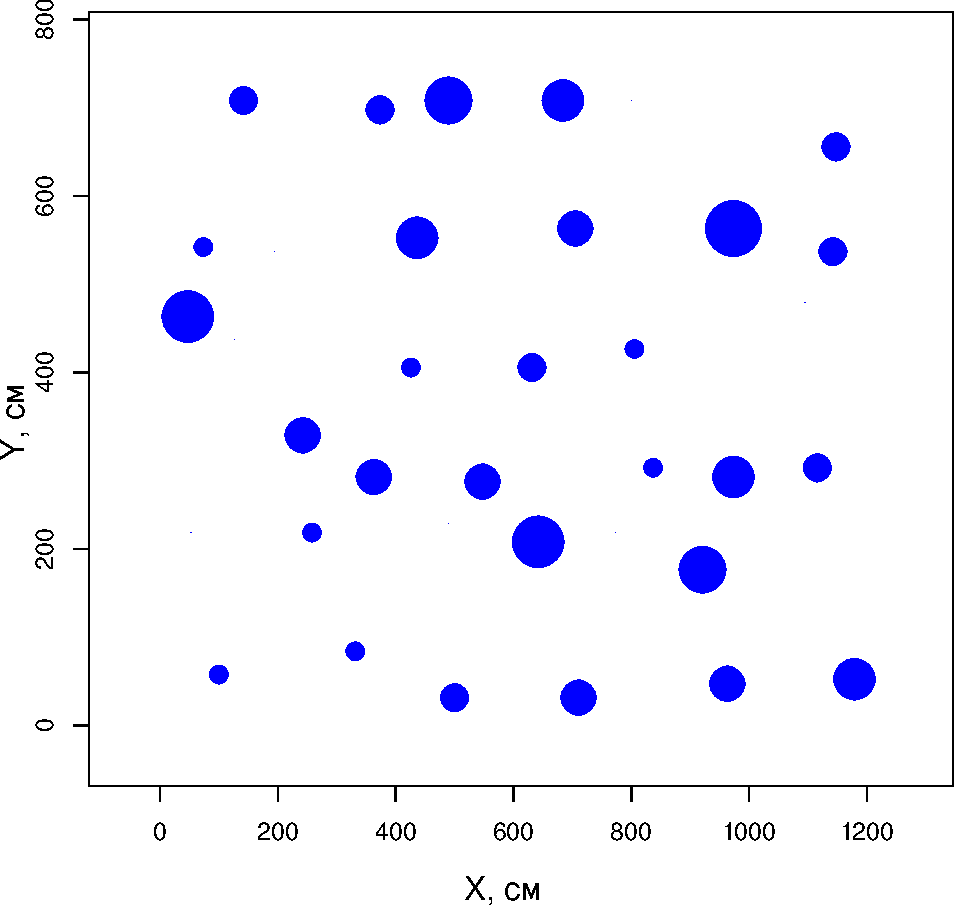
\includegraphics[width=49mm]{./microdistribution/Yarnyshnaya_N_Macoma_bubbles.pdf}
	\end{center}
	\end{minipage}
\end{figure}
\end{frame}






\begin{frame}{Микрораспределение {\it Macoma~balthica}}
\framesubtitle{бухта Дровяная, Пала-губа}
% микрораспределение по обилию
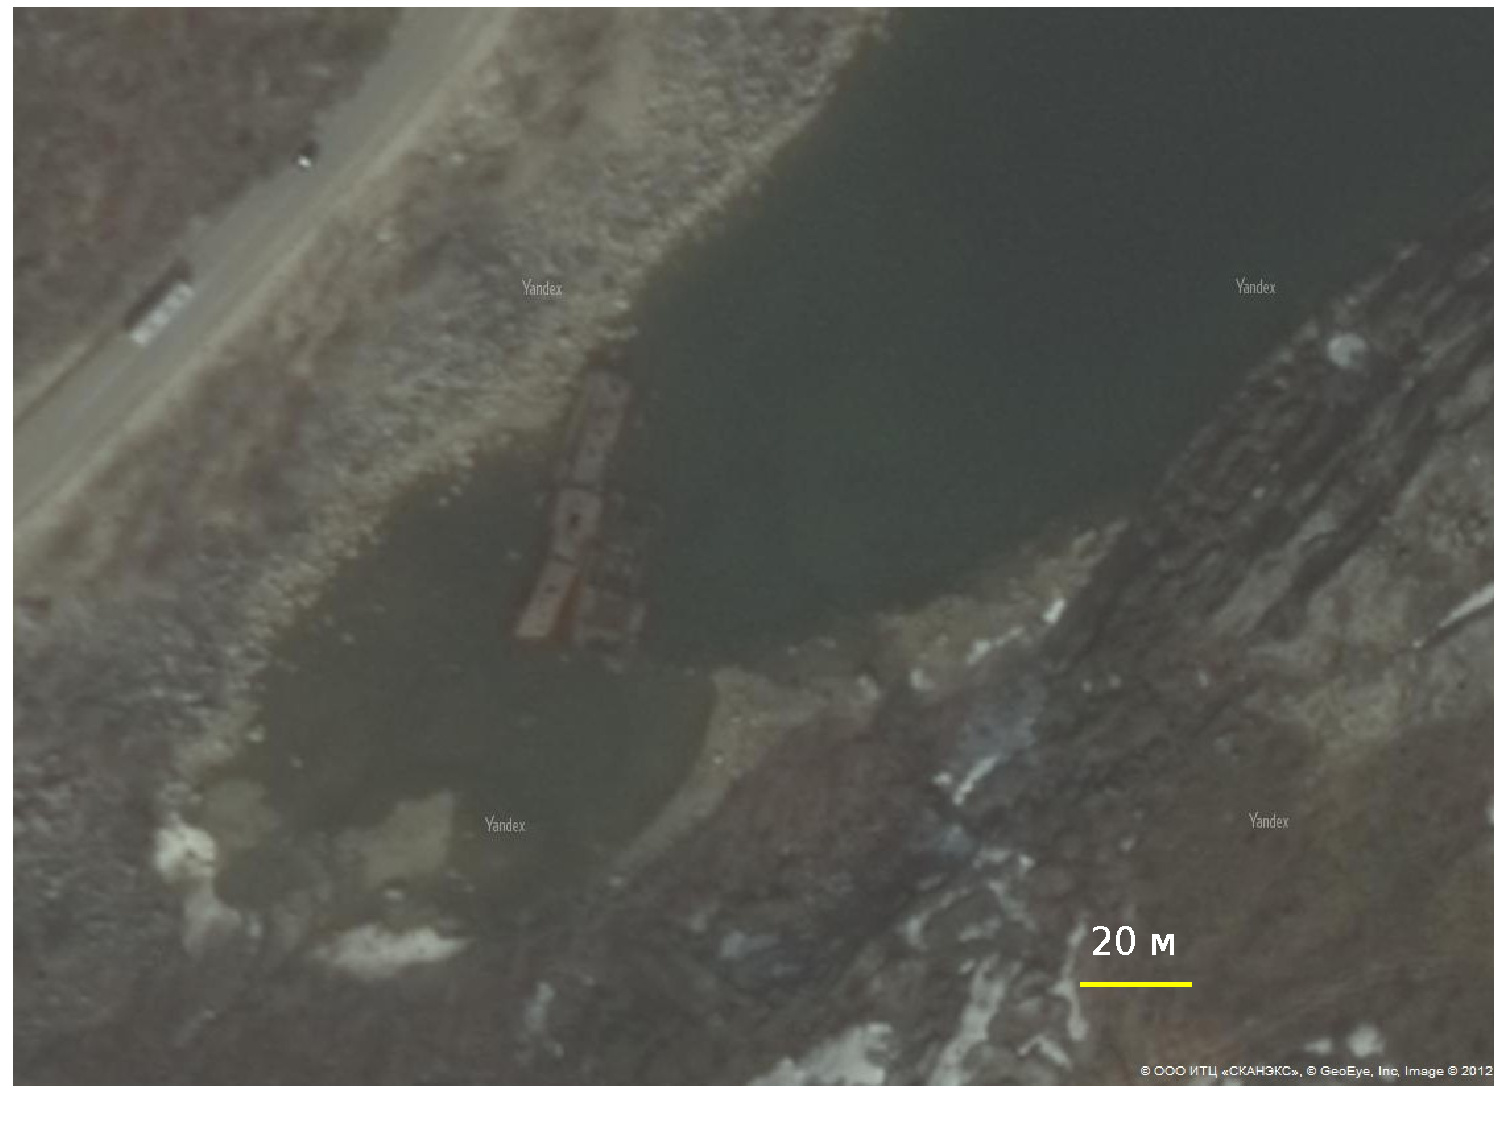
\includegraphics[width=100mm]{./Pala_snimok.pdf}

(спутниковый снимок, maps.yandex.ru)
\end{frame}

\begin{frame}{Микрораспределение {\it Macoma~balthica}}
\framesubtitle{Схема Пала-губы и исследованный полигон}
% микрораспределение по обилию
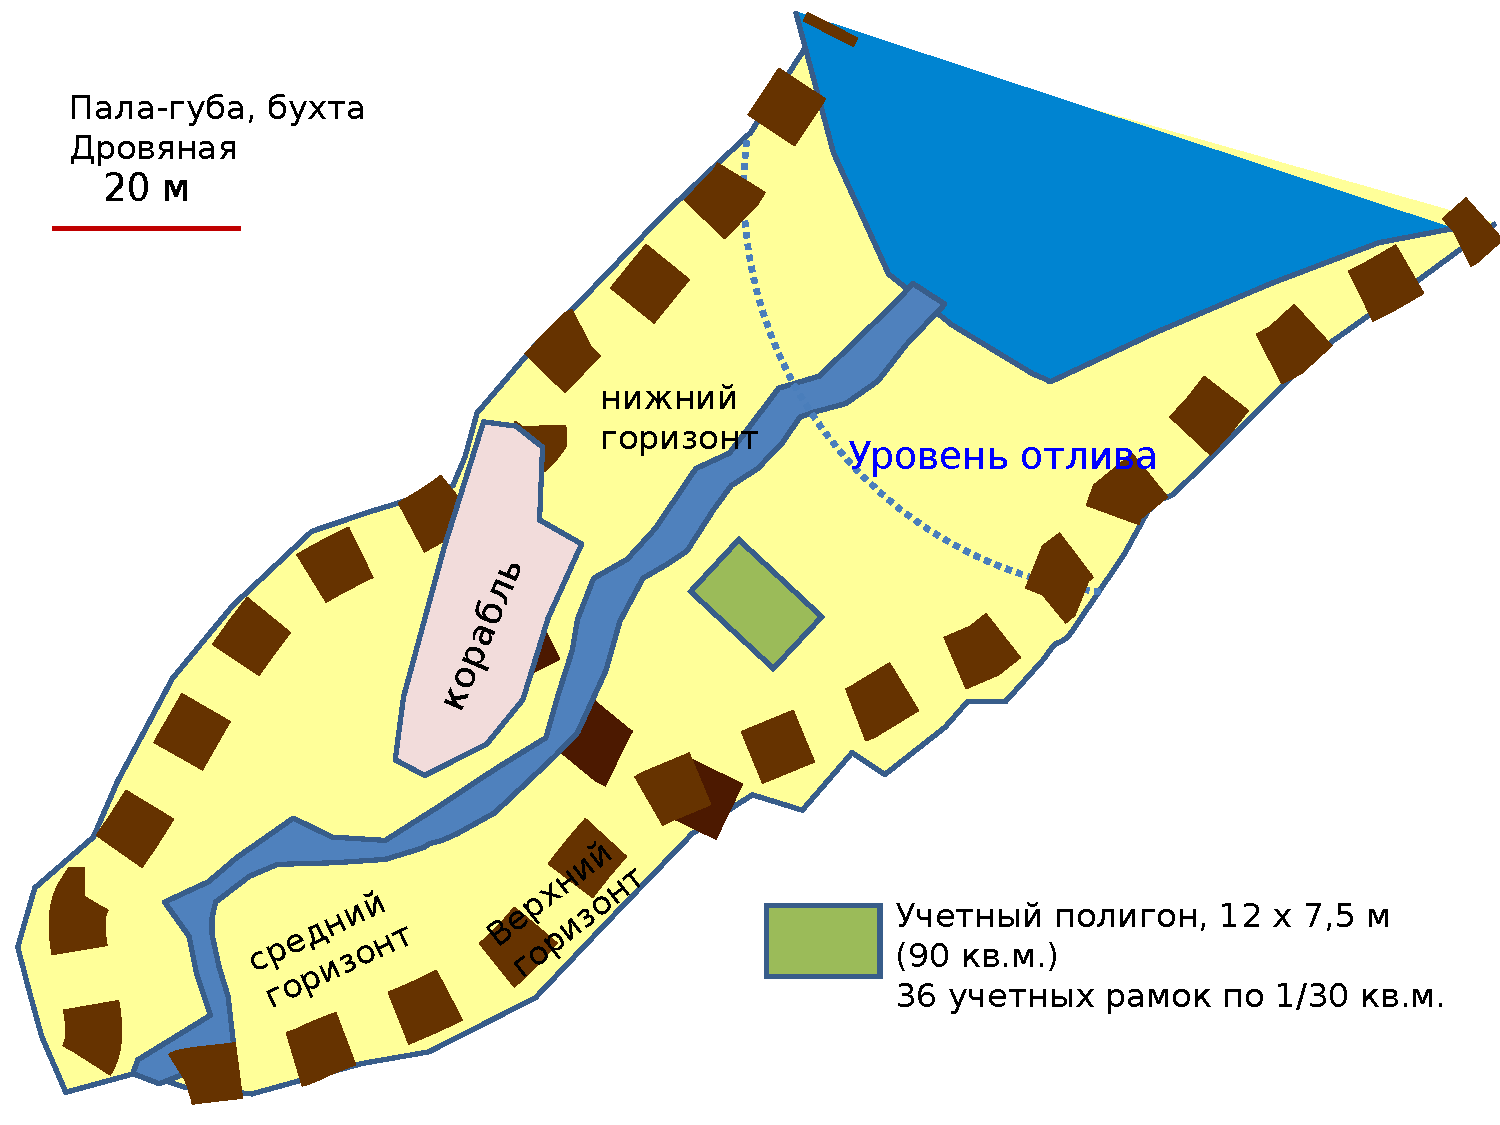
\includegraphics[width=100mm]{./Pala_shema_midist.pdf}
\end{frame}

\begin{frame}{Микрораспределение {\it Macoma~balthica}}
\framesubtitle{Пала-губа: Распределение маком по суммарной численности}
% микрораспределение по обилию
\begin{center}
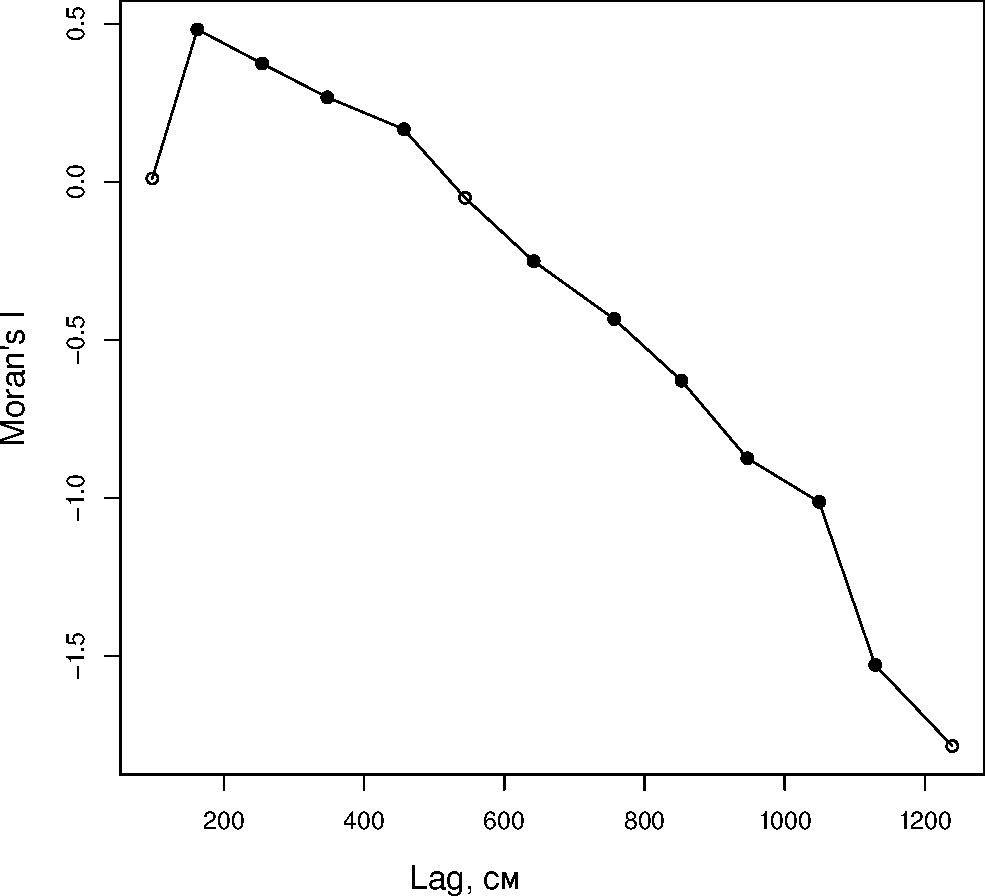
\includegraphics[width=49mm]{./microdistribution/Pala_moran_N_Macoma_balthica_.pdf}
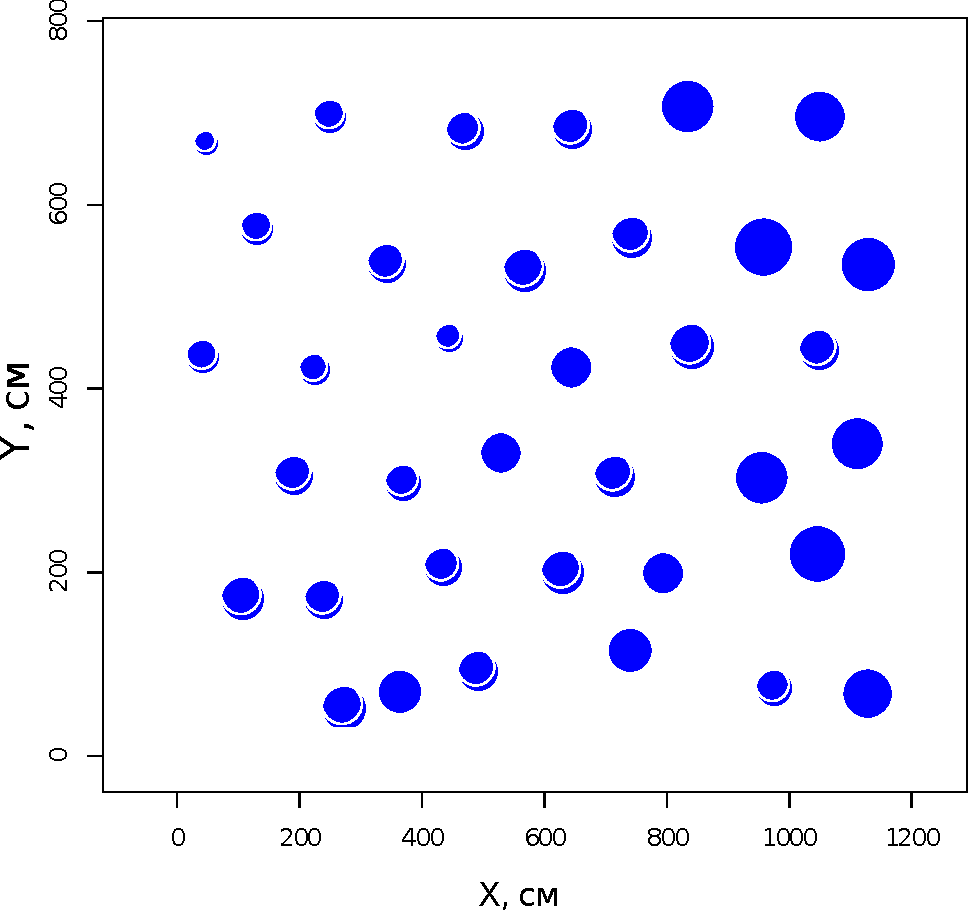
\includegraphics[width=49mm]{./microdistribution/Pala_N_Macoma_bubbles.pdf}
\end{center}
\end{frame}

\begin{frame}{Размерная структура {\it Macoma~balthica} в поселении нижней литорали Пала-губы}
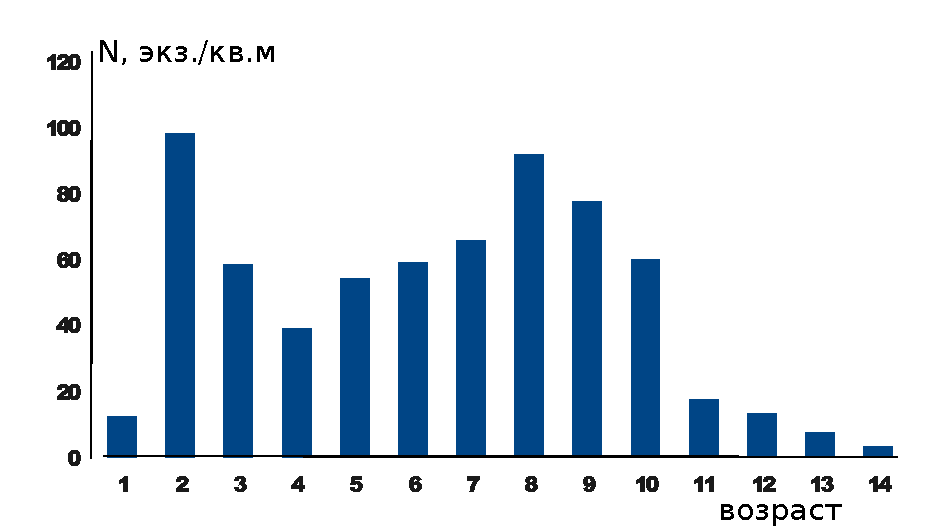
\includegraphics[width=80mm]{./microdistribution/Pala07_autumn_sizestr.pdf}
\end{frame}

\begin{frame}{Микрораспределение {\it Macoma~balthica}}
\framesubtitle{Пала-губа: Распределение маком доминирующих возрастных групп}
% микрораспределение возрастов
возрастная группа 2+
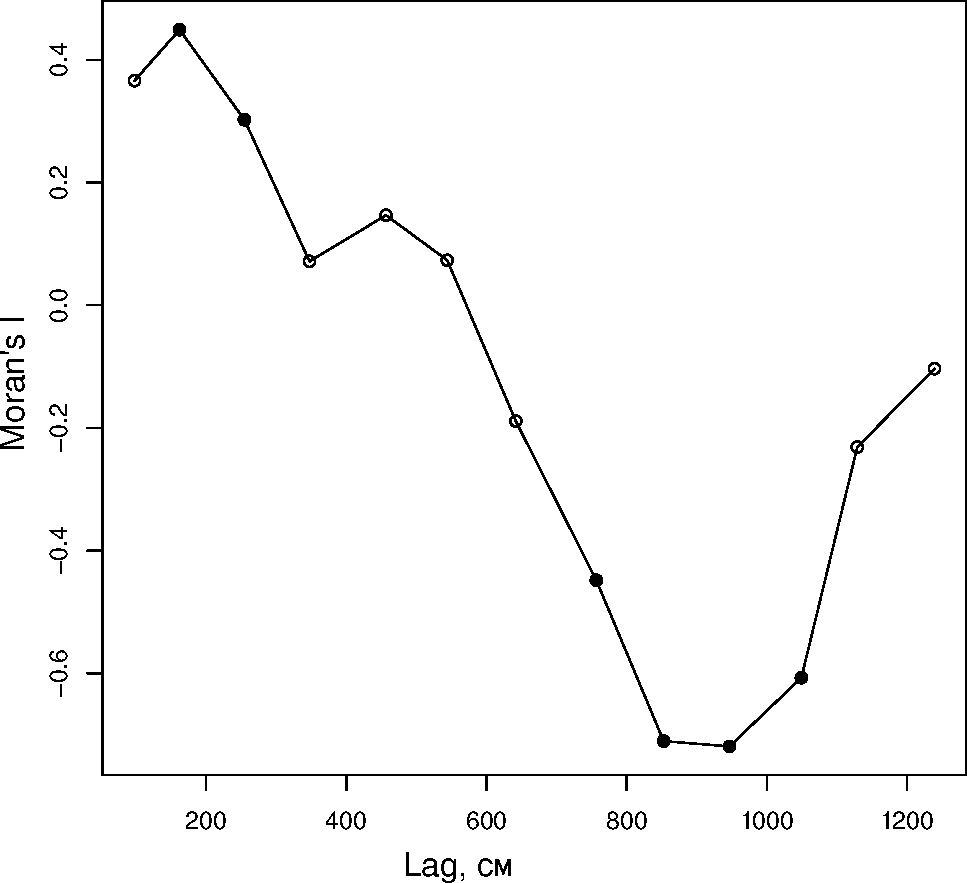
\includegraphics[width=35mm]{./microdistribution/Pala_macoma_age_N2_.pdf}
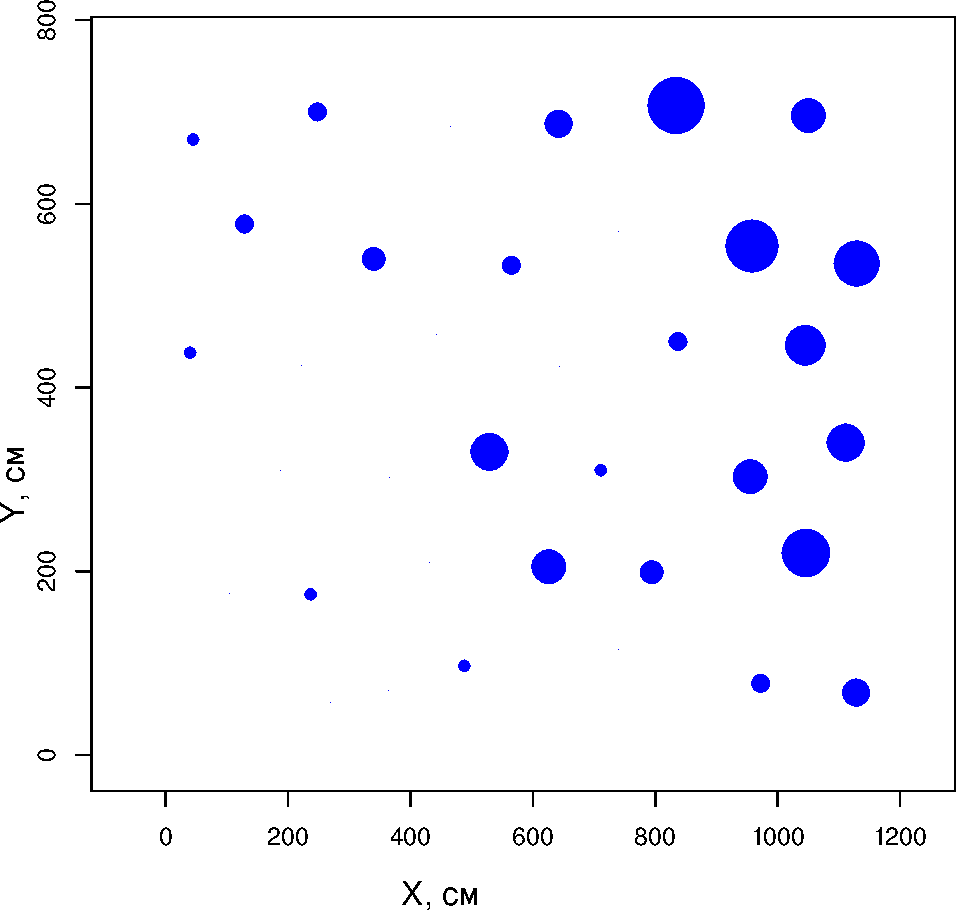
\includegraphics[width=35mm]{./microdistribution/Pala_macoma_age_bubb_N2_.pdf}

возрастная группа 8+
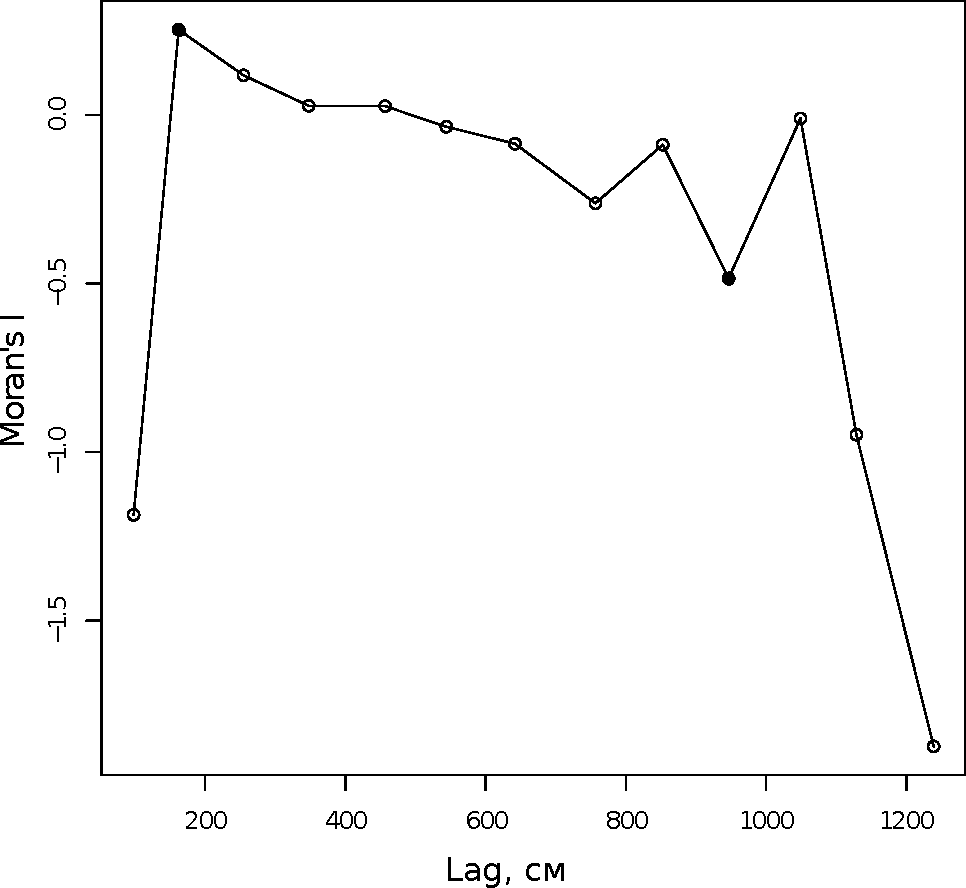
\includegraphics[width=35mm]{./microdistribution/Pala_macoma_age_N8_.pdf}
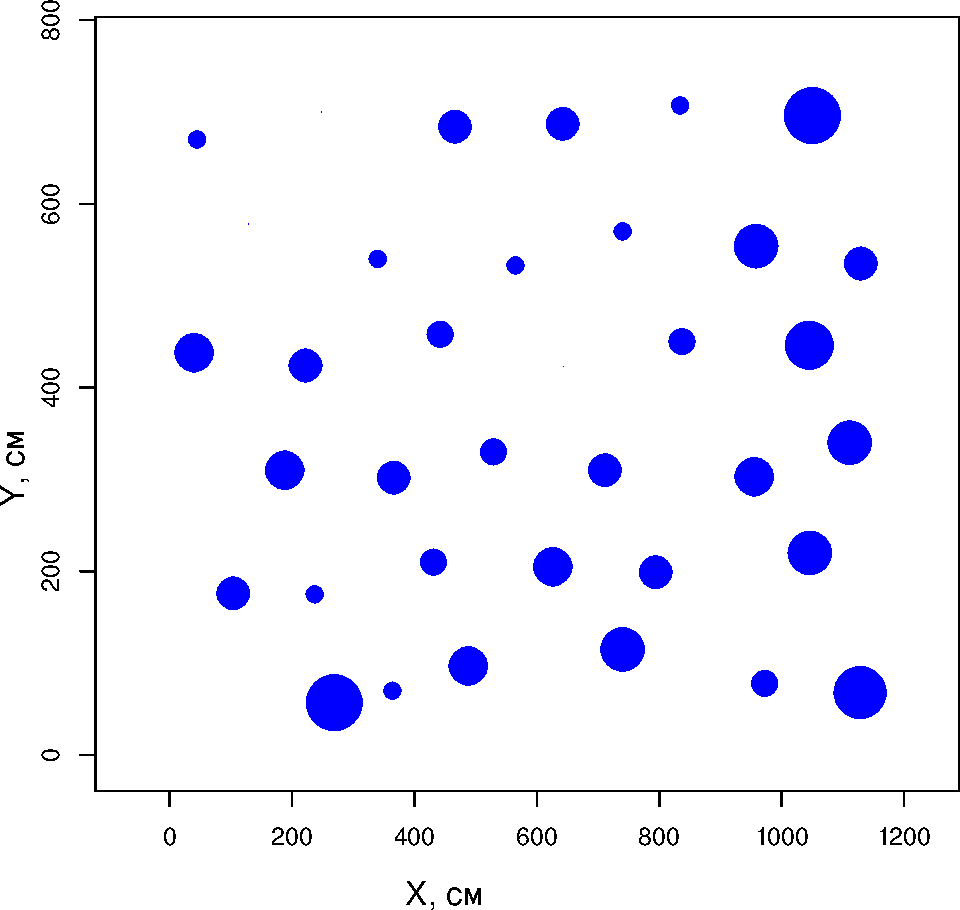
\includegraphics[width=35mm]{./microdistribution/Pala_macoma_age_bubb_N8_.pdf}

\end{frame}

\begin{frame}{Микрораспределение {\it Macoma~balthica}}
\framesubtitle{Распределение маком доминирующих возрастных групп}
% микрораспределение возрастов схема
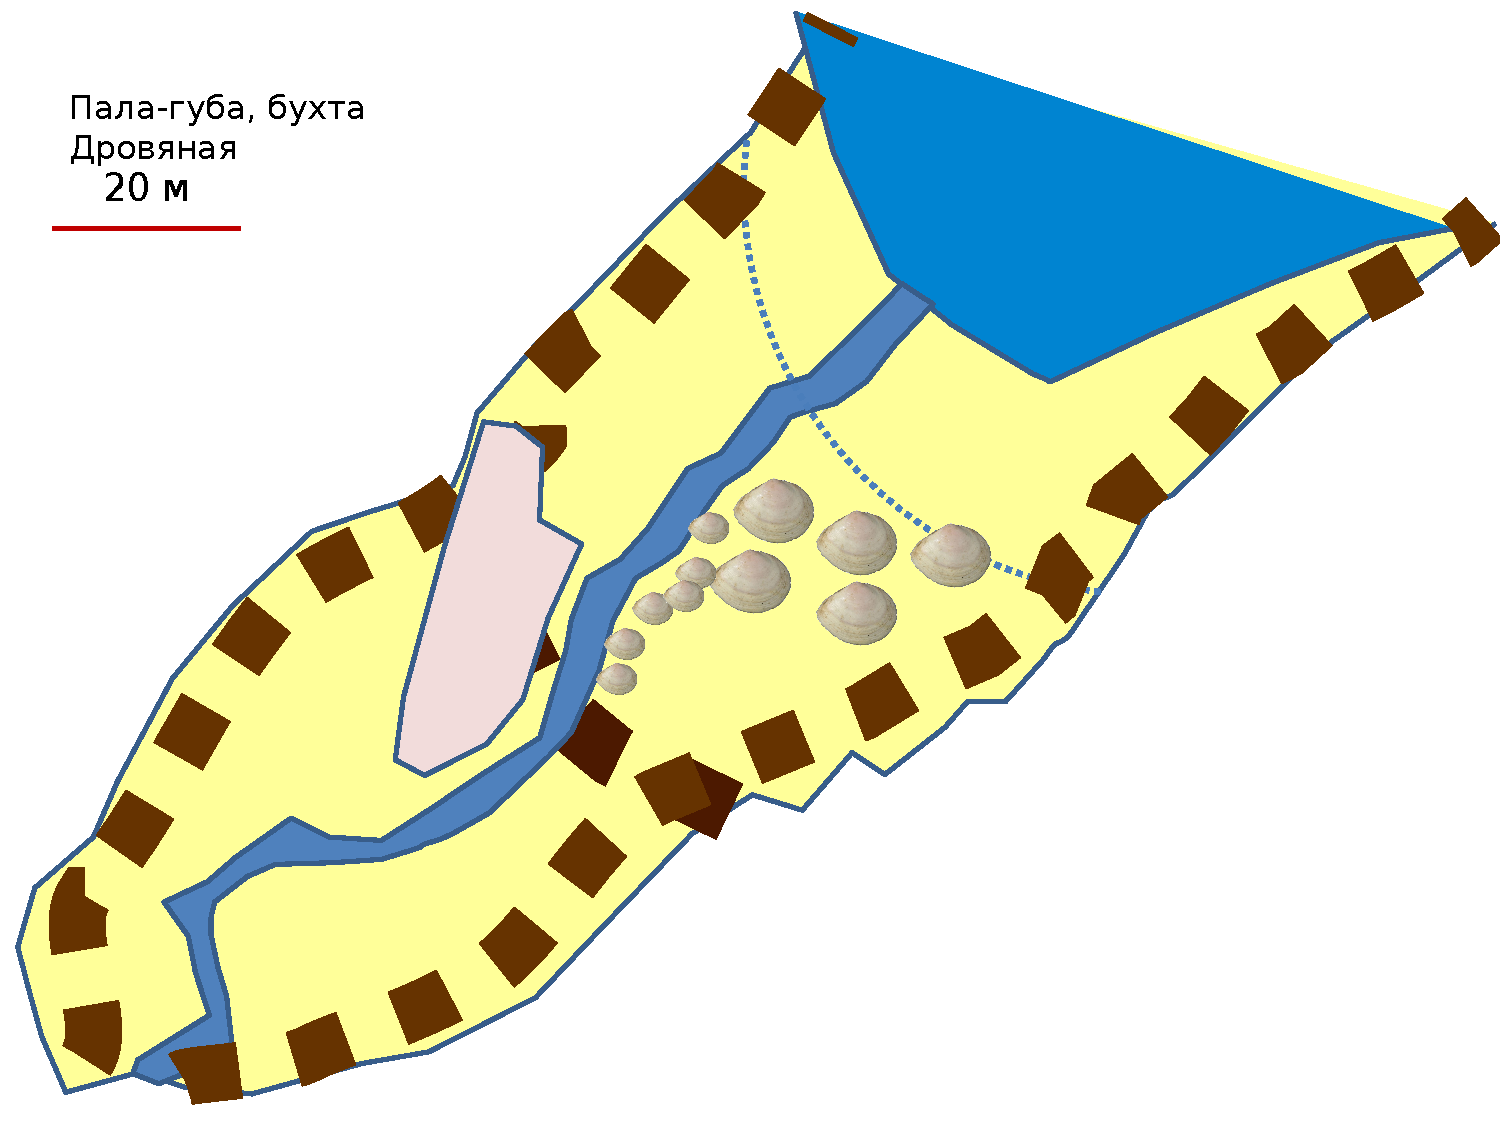
\includegraphics[width=100mm]{./Pala_distribution.pdf}
\end{frame}







	\section{Обилие {\it Macoma~balthica}}
\begin{frame}{Варьирование обилия {\it Macoma~balthica} на исследованных участках}
%Наверное по пробам более показательно - показать размах. Или не гисторгамму, а боксплот.
%Можно ведь для моря или для каждого участка...
\begin{figure}
\begin{minipage}[b]{.49\linewidth}
	\begin{center}
Белое море
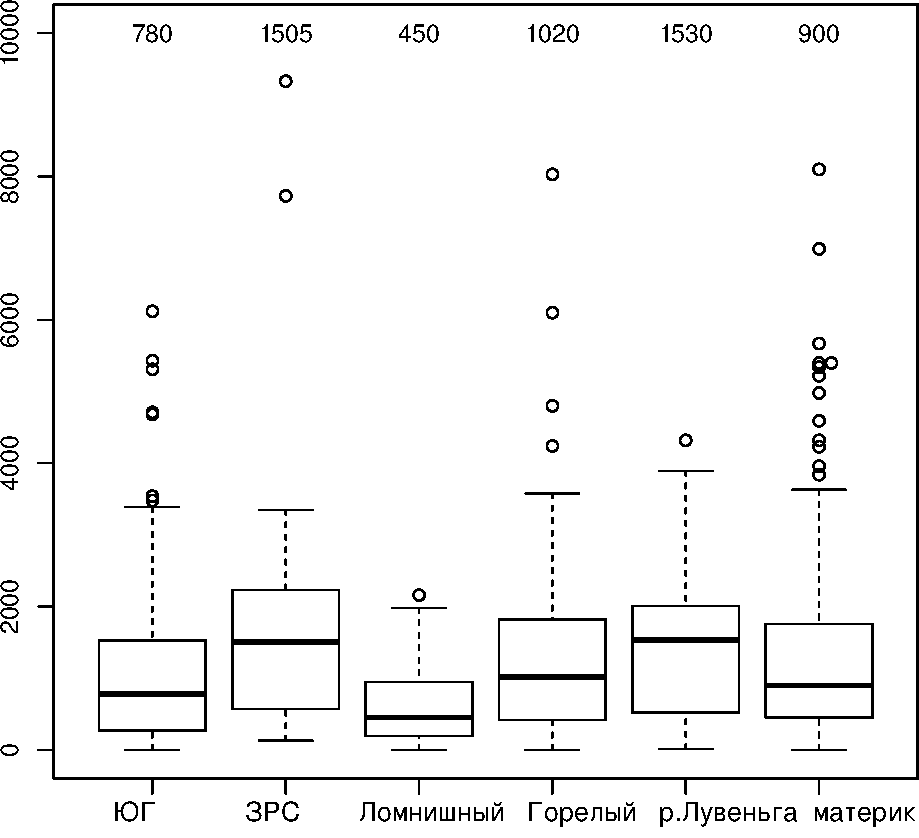
\includegraphics[width=49mm]{./N_all/N2_area_White1.pdf}
\end{center}
	\end{minipage}
	\hfil %Это пружинка отодвигающая рисунки друг от друга
	\begin{minipage}[b]{.49\linewidth}
\begin{center}
Баренцево море
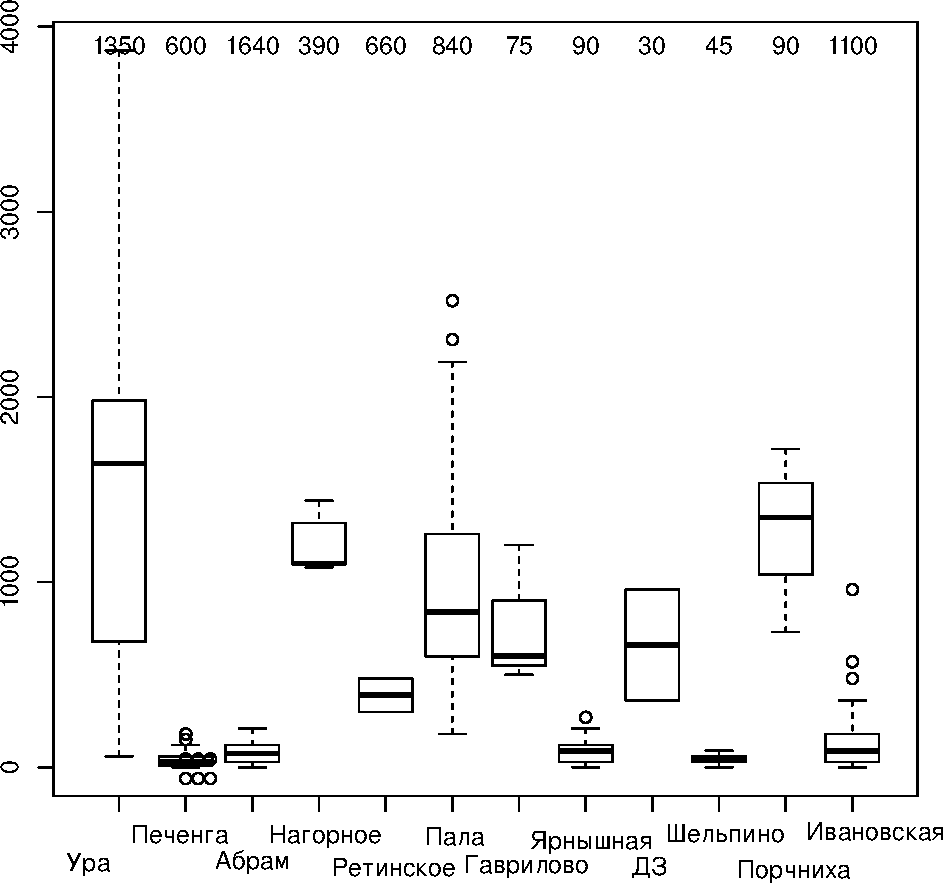
\includegraphics[width=49mm]{./N_all/N2_area_Barents1.pdf}
	\end{center}
	\end{minipage}
\end{figure}
\end{frame}


\begin{frame}{Обилие {\it Macoma~balthica} в различных районах исследования}
\begin{center}
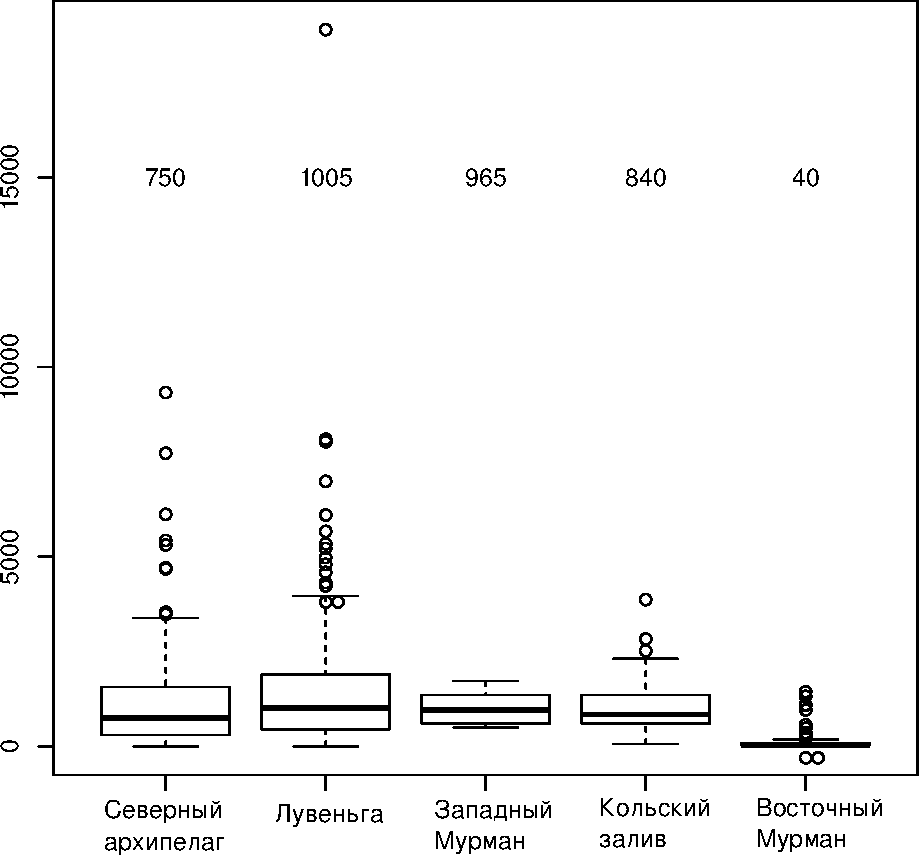
\includegraphics[width=70mm]{./N_all/N2_region1.pdf}
\end{center}
\end{frame}


\begin{frame}{Динамика обилия {\it Macoma~balthica}}
\framesubtitle{Белое море}
\begin{figure}
	\begin{minipage}[b]{.3\linewidth}
	\begin{center}
\tiny{Эстуарий р.~Лувеньги}
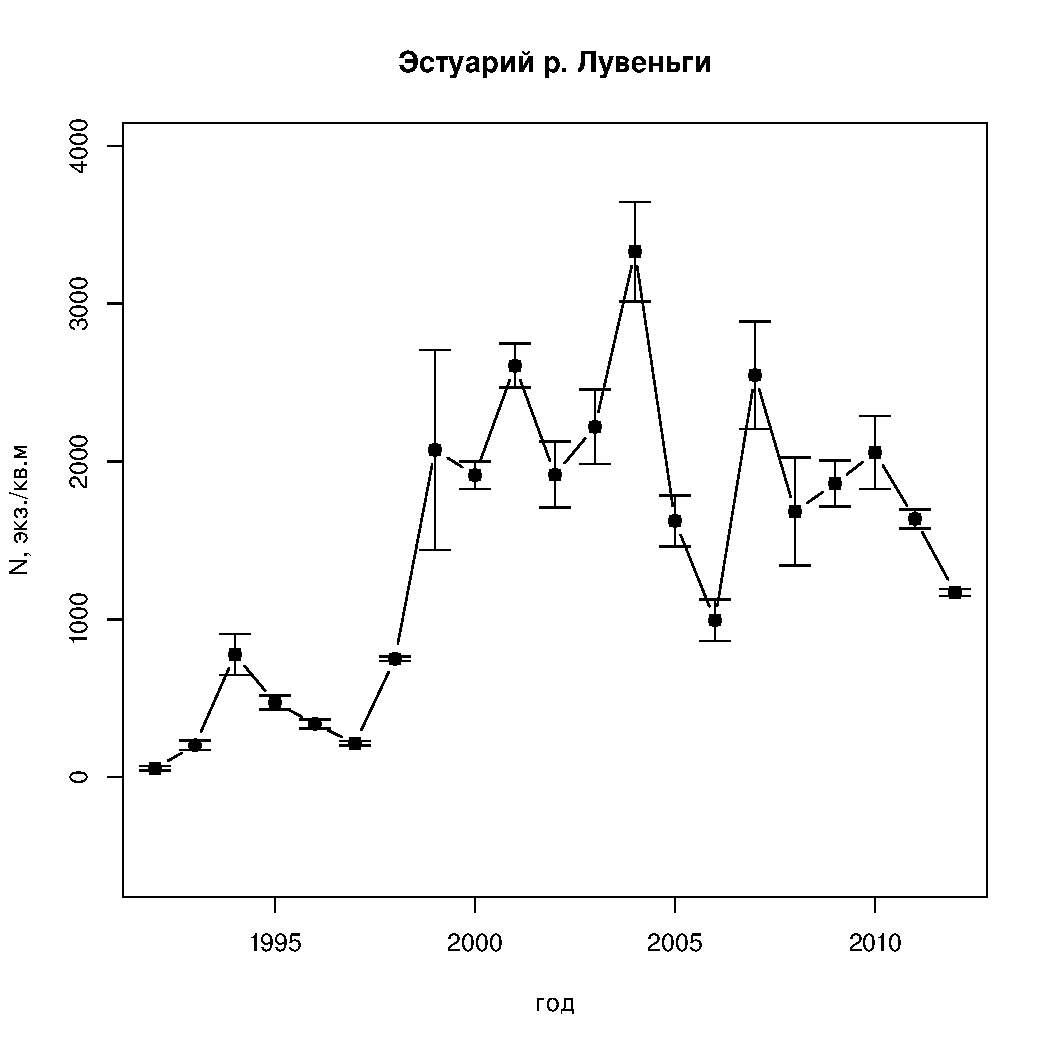
\includegraphics[width=30mm]{../White_Sea/Estuatiy_Luvenga/N2_dynamic.pdf}
	\end{center}
	\end{minipage}
\hfil %Это пружинка отодвигающая рисунки друг от друга
	\begin{minipage}[b]{.3\linewidth}
	\begin{center}
\tiny{о.~Горелый}
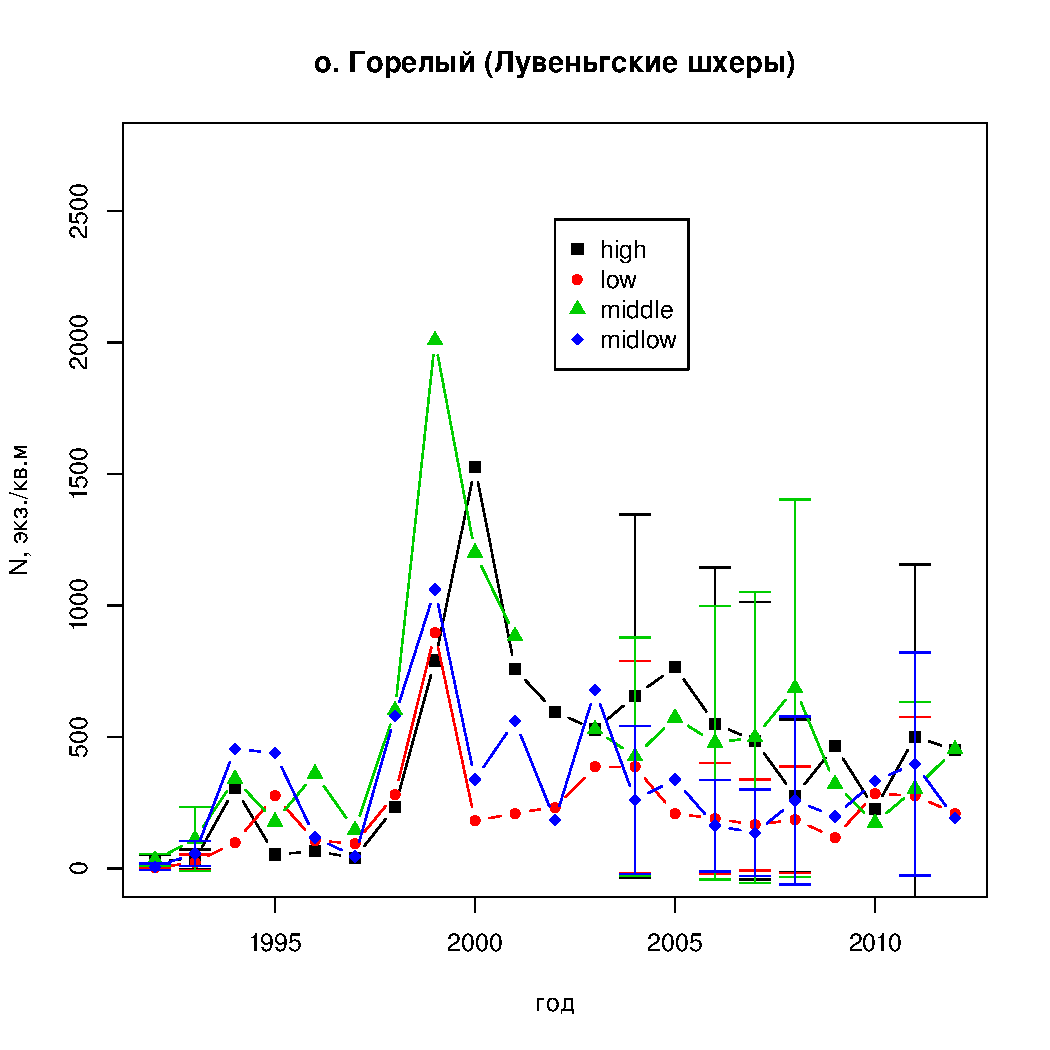
\includegraphics[width=30mm]{../White_Sea/Luvenga_Goreliy/N2_dynamic.pdf}
	\end{center}
	\end{minipage}
\hfil %Это пружинка отодвигающая рисунки друг от друга
	\begin{minipage}[b]{.3\linewidth}
	\begin{center}
\tiny{материковая литораль, Лувеньга}
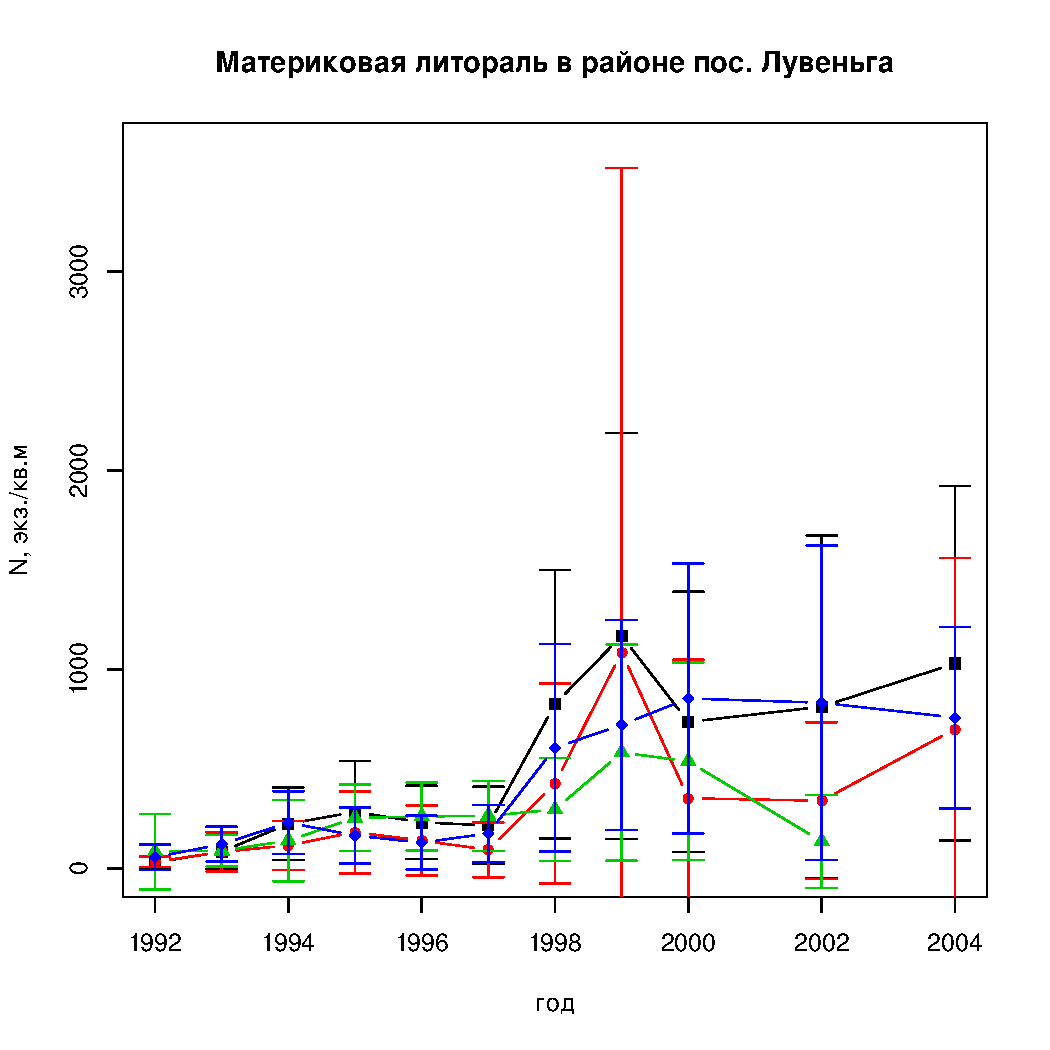
\includegraphics[width=30mm]{../White_Sea//Luvenga_II_razrez/N2_dynamic.pdf}
	\end{center}
	\end{minipage}
	\begin{minipage}[b]{.3\linewidth}
	\begin{center}
\tiny{ЗРС о.~Ряшков}
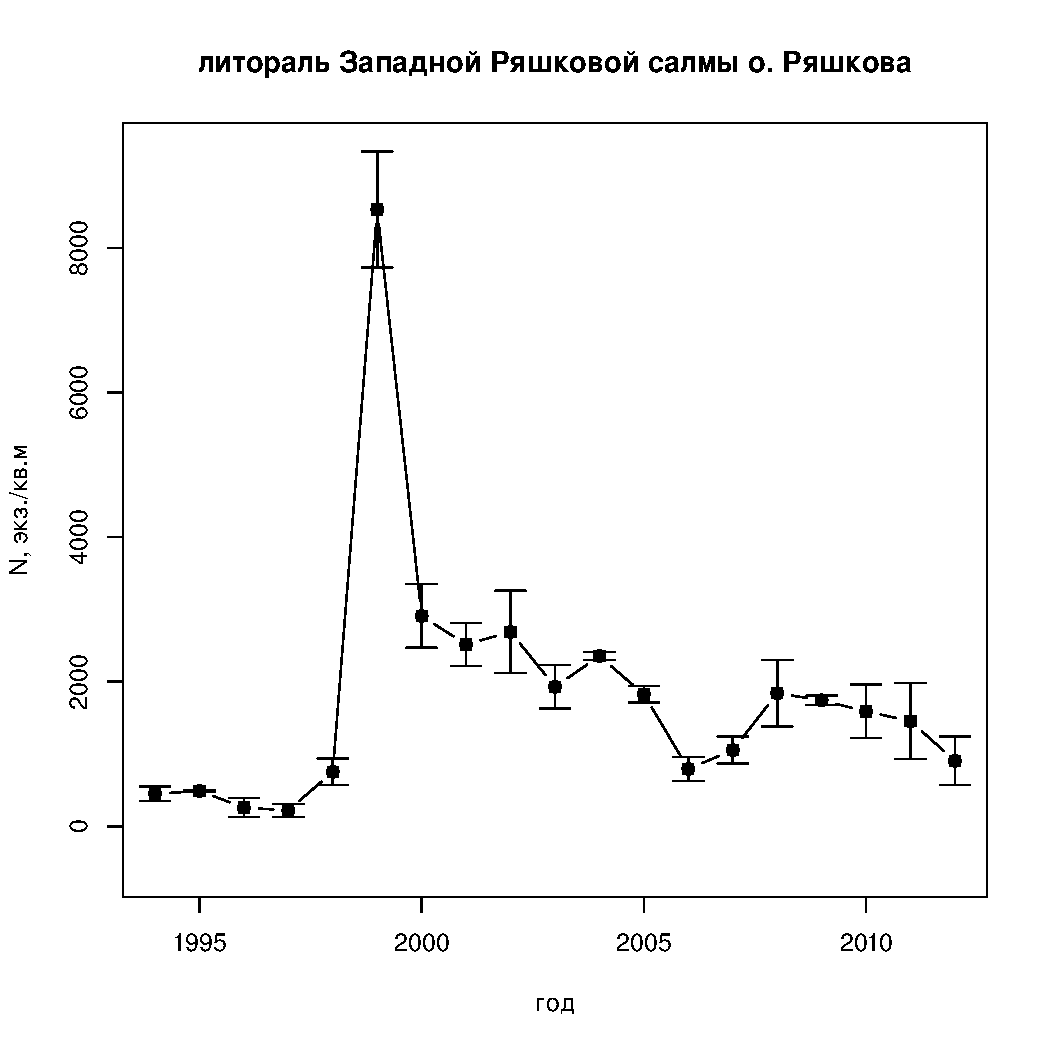
\includegraphics[width=30mm]{../White_Sea/Ryashkov_ZRS/N2_dynamic.pdf}
	\end{center}
	\end{minipage}
\hfil %Это пружинка отодвигающая рисунки друг от друга
	\begin{minipage}[b]{.3\linewidth}
	\begin{center}
\tiny{Южная губа о.~Ряшков}
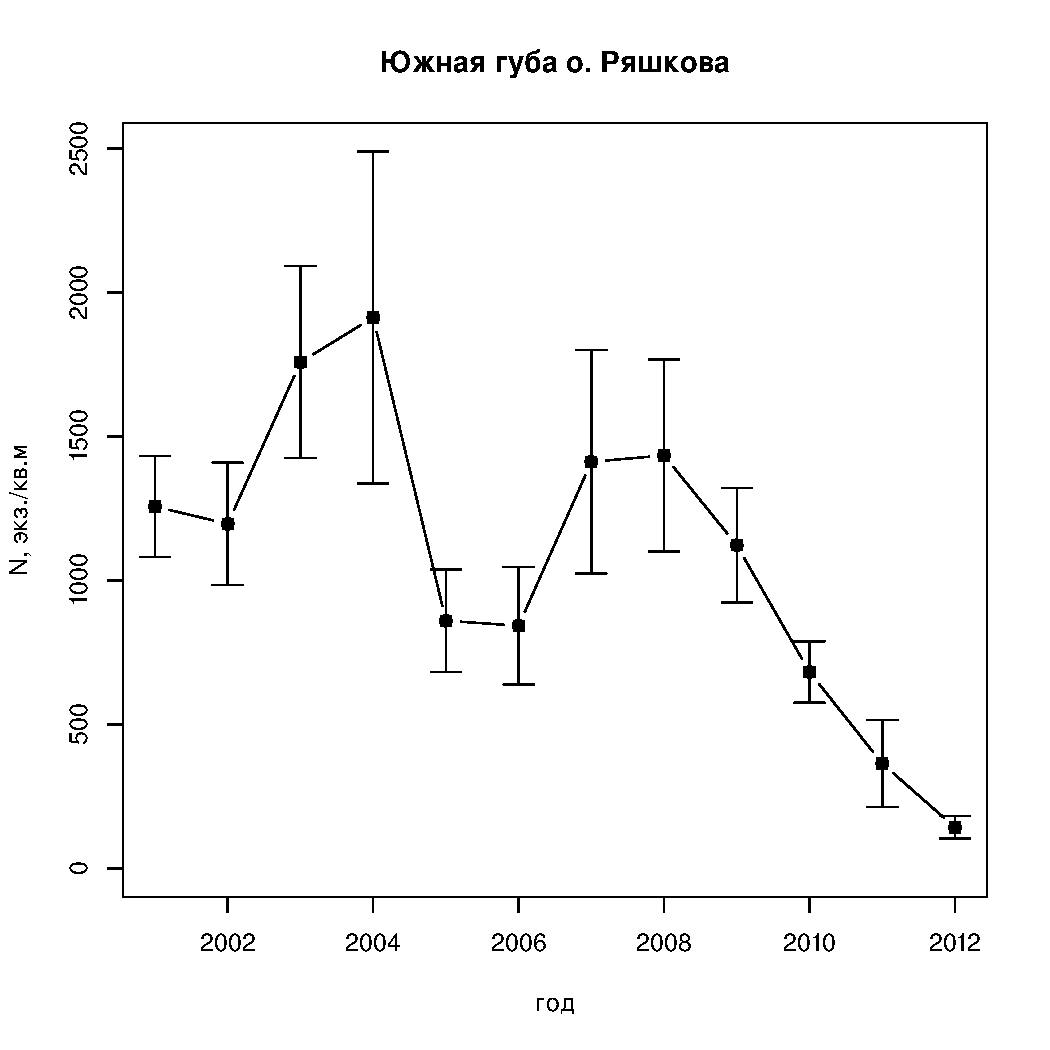
\includegraphics[width=30mm]{../White_Sea/Ryashkov_YuG/N2_dynamic.pdf}
	\end{center}
	\end{minipage}
\hfil %Это пружинка отодвигающая рисунки друг от друга
	\begin{minipage}[b]{.3\linewidth}
	\begin{center}
\tiny{о.Ломнишный}
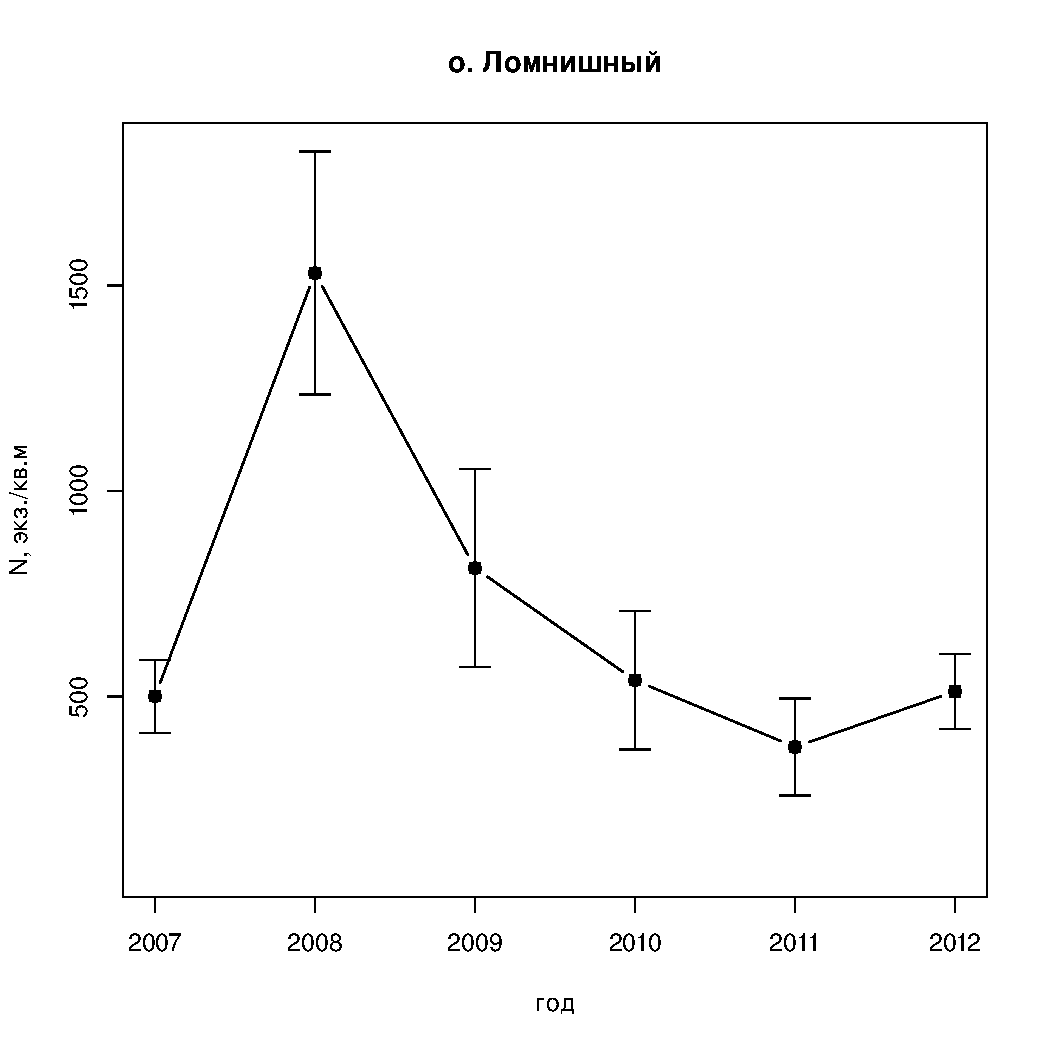
\includegraphics[width=30mm]{../White_Sea/Lomnishniy/N2_dynamic.pdf}
	\end{center}
	\end{minipage}
\end{figure}
\end{frame}

\begin{frame}{Динамика обилия {\it Macoma~balthica}}
\framesubtitle{Баренцево море, Дальний Пляж губы Дальнезеленецкая}
\begin{center}
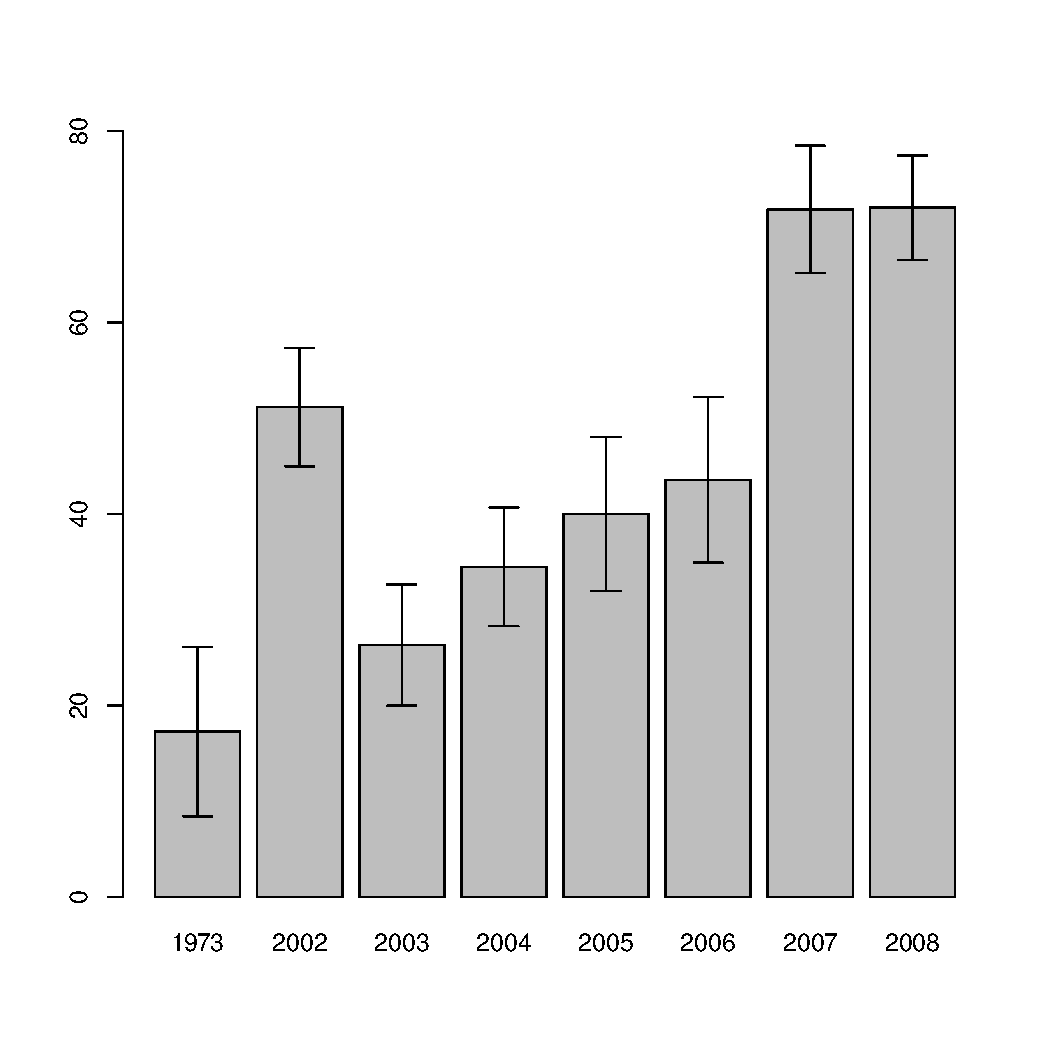
\includegraphics[width=70mm]{../Barenc_Sea/Dalnezeleneckaya/N_dynamic_with_Agarova.pdf}
\end{center}
\tiny{$1973$ год -- по данным Агаровой и др., 1976.}
\end{frame}

	\section{Размерная структура {\it Macoma~balthica}}
\begin{frame}{Классификация типов размерных структур}
% круто бы мдс или ГК по процентной РС
\end{frame}

	
\begin{frame}{Динамика размерной структуры {\it Macoma~balthica}}
%непонятно как забить в один-два-три слайда
Эстуарий р. Лувеньги. Нерегулярное пополнение
\begin{figure}[h]
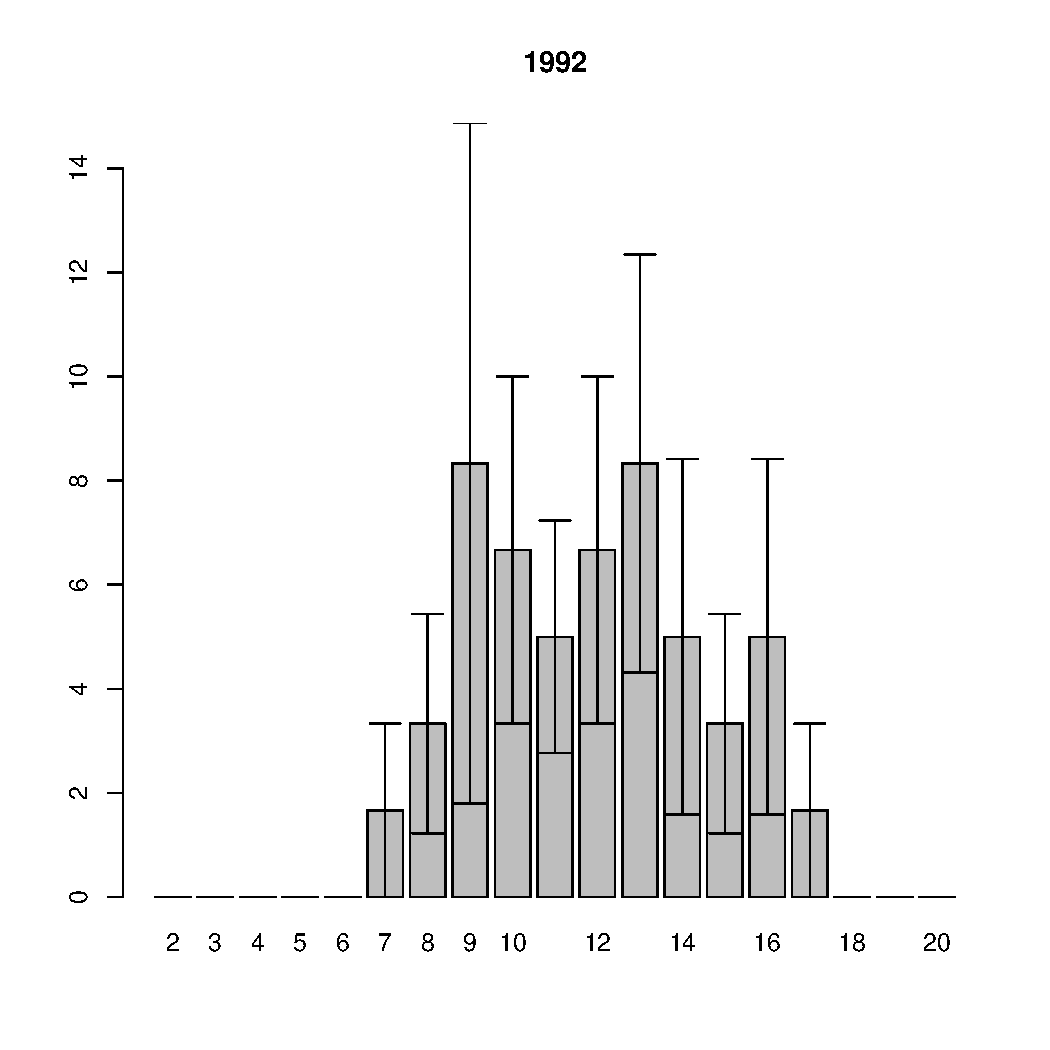
\includegraphics[width=14mm]{../White_Sea/Estuatiy_Luvenga/sizestr2_1992_.pdf}
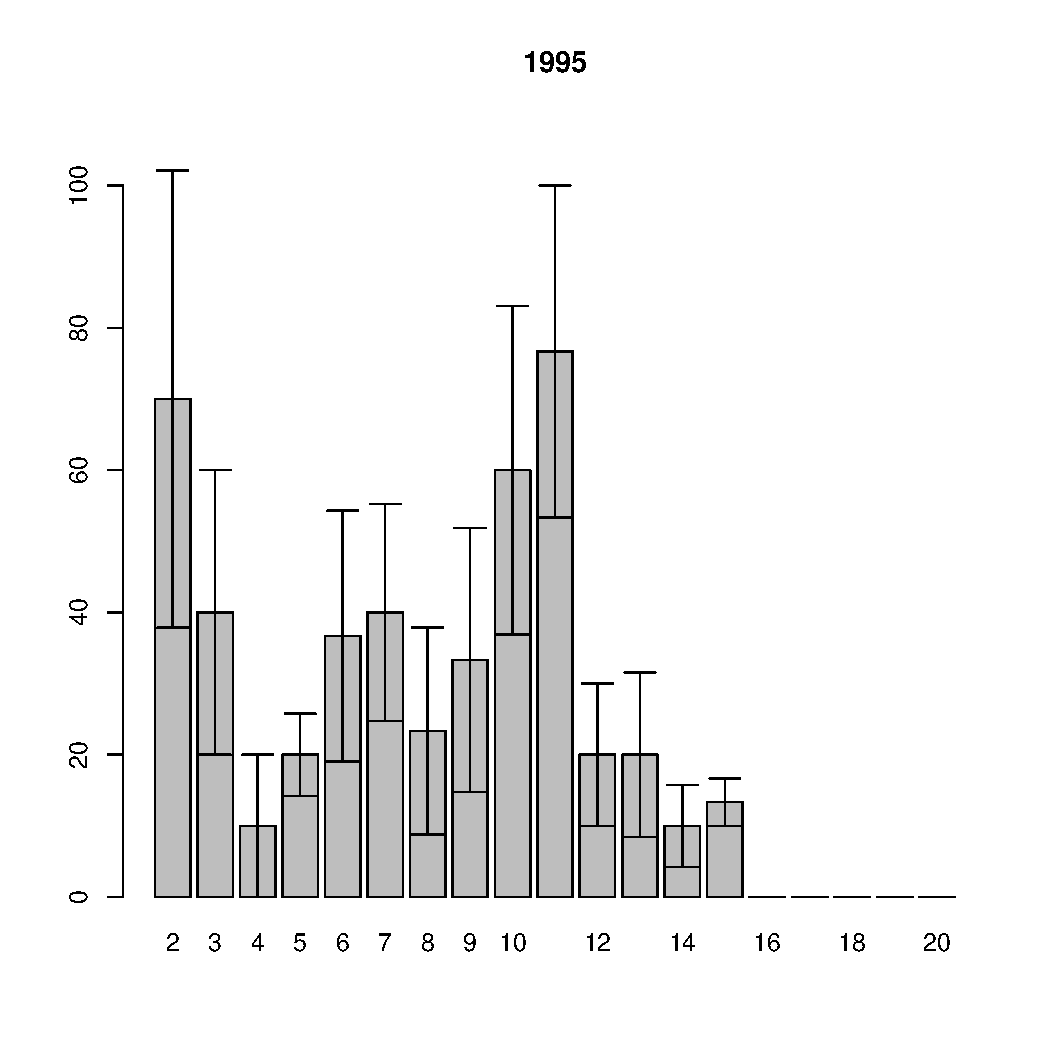
\includegraphics[width=14mm]{../White_Sea/Estuatiy_Luvenga/sizestr2_1995_.pdf}
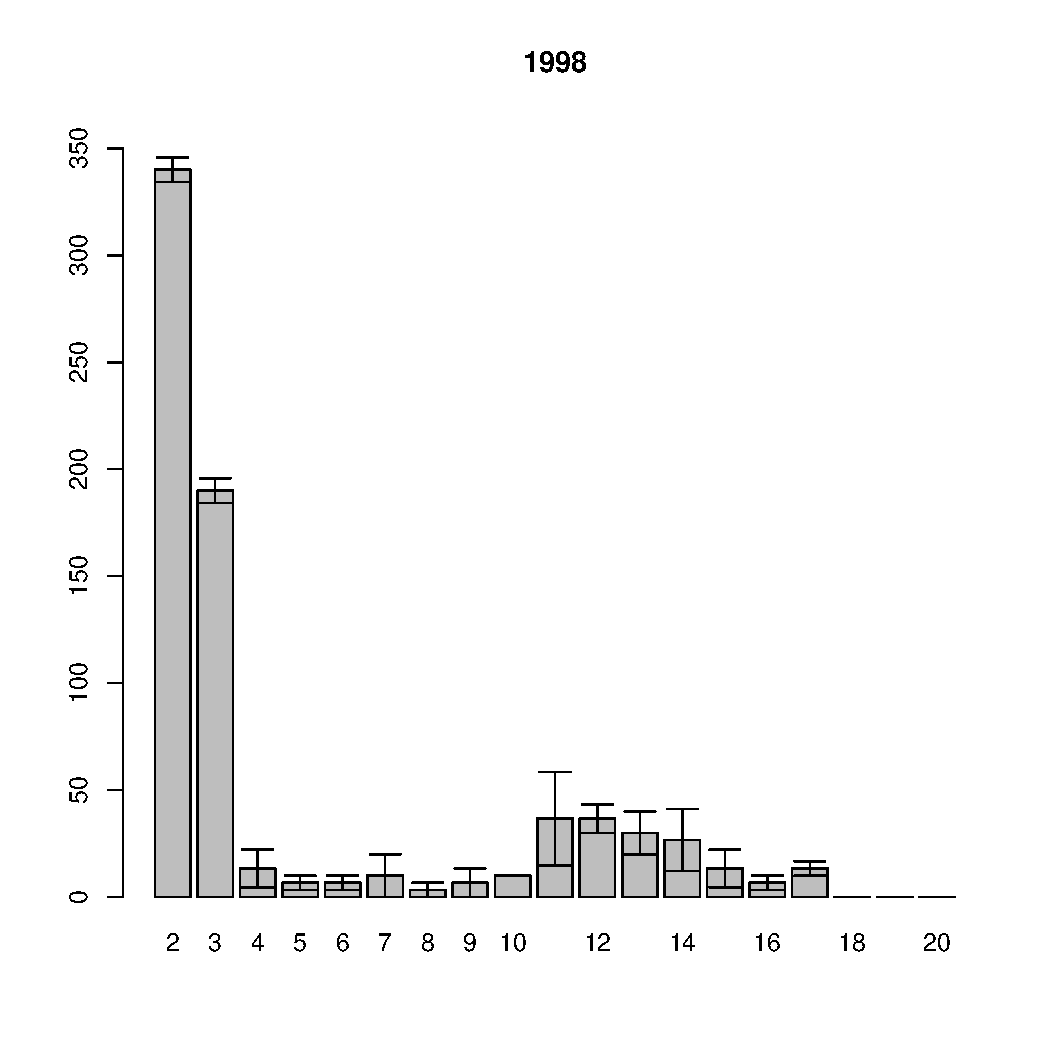
\includegraphics[width=14mm]{../White_Sea/Estuatiy_Luvenga/sizestr2_1998_.pdf}
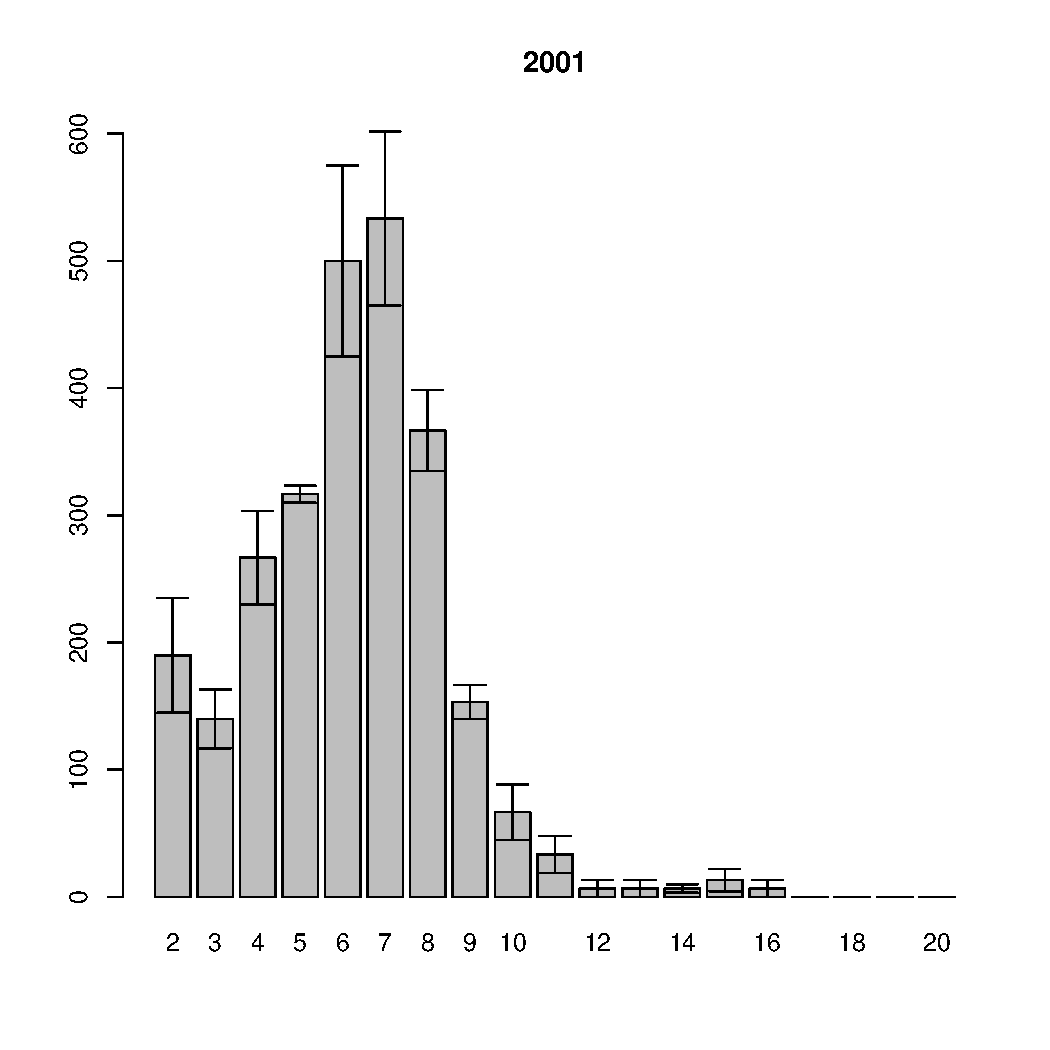
\includegraphics[width=14mm]{../White_Sea/Estuatiy_Luvenga/sizestr2_2001_.pdf}
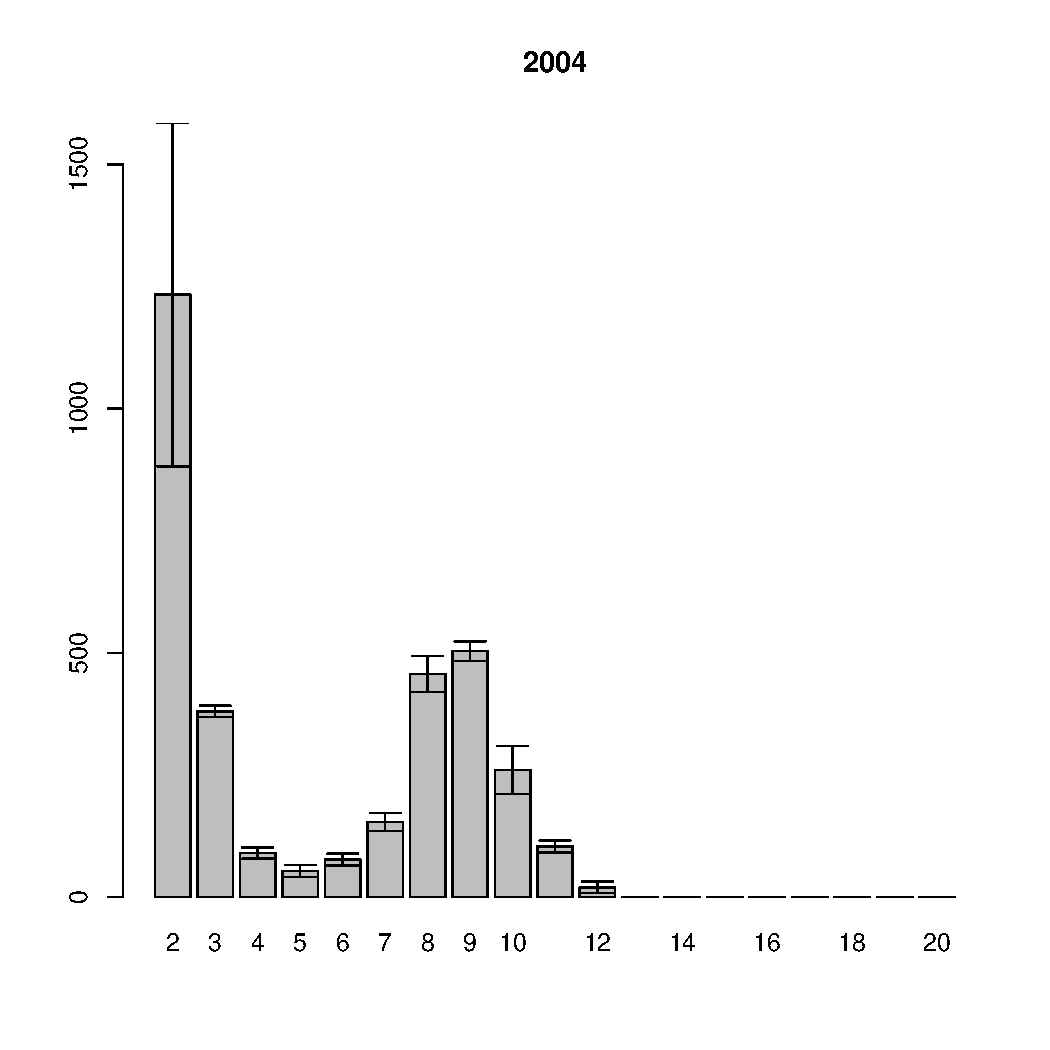
\includegraphics[width=14mm]{../White_Sea/Estuatiy_Luvenga/sizestr2_2004_.pdf}
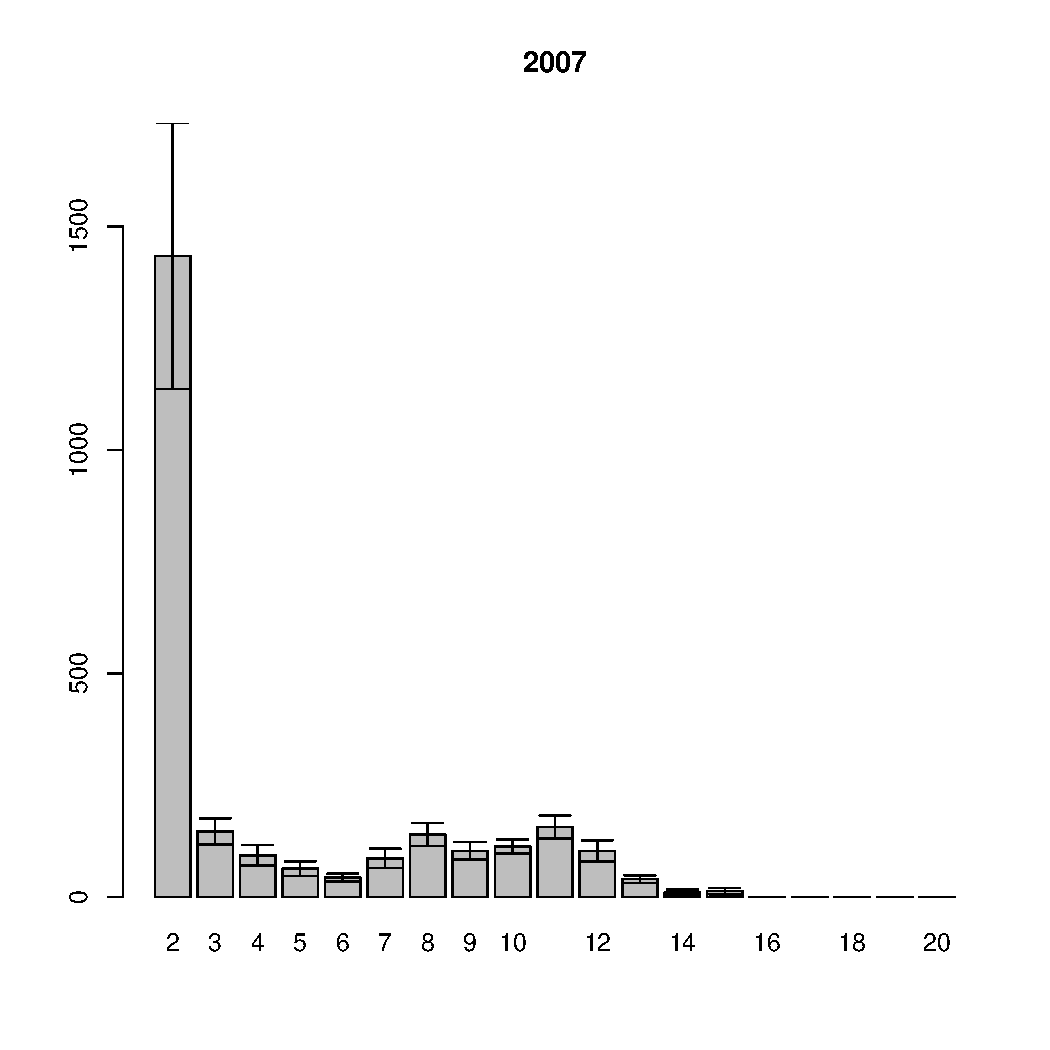
\includegraphics[width=14mm]{../White_Sea/Estuatiy_Luvenga/sizestr2_2007_.pdf}
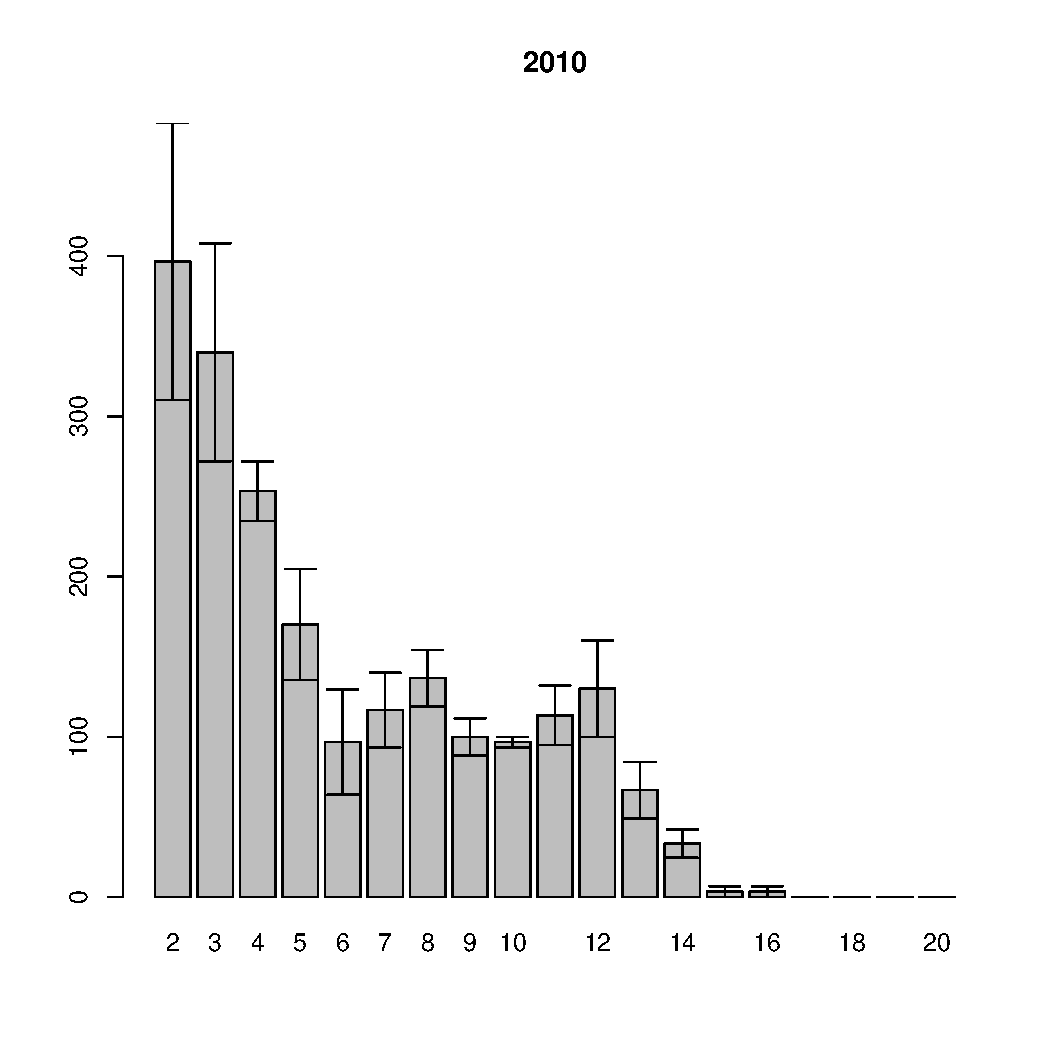
\includegraphics[width=14mm]{../White_Sea/Estuatiy_Luvenga/sizestr2_2010_.pdf}
\end{figure}
\begin{figure}[h]
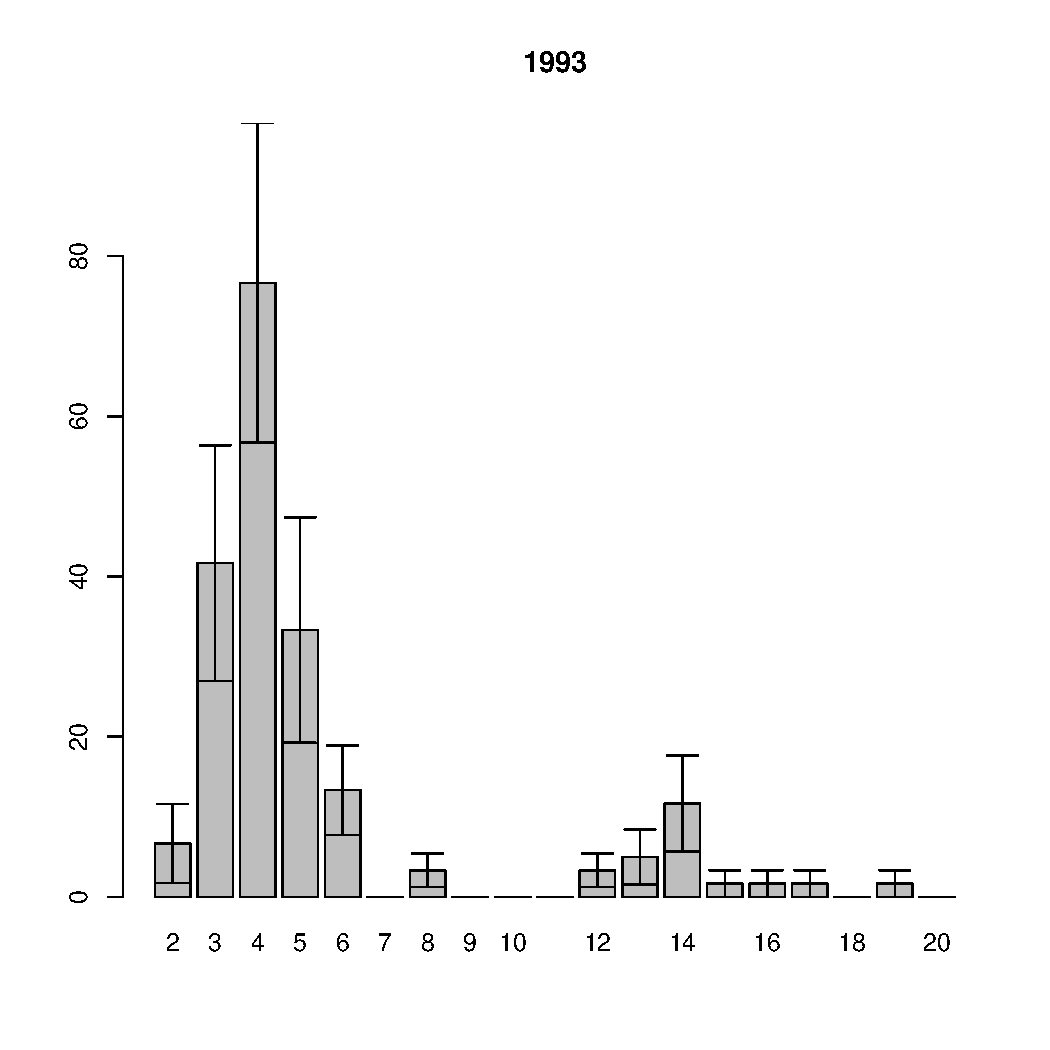
\includegraphics[width=14mm]{../White_Sea/Estuatiy_Luvenga/sizestr2_1993_.pdf}
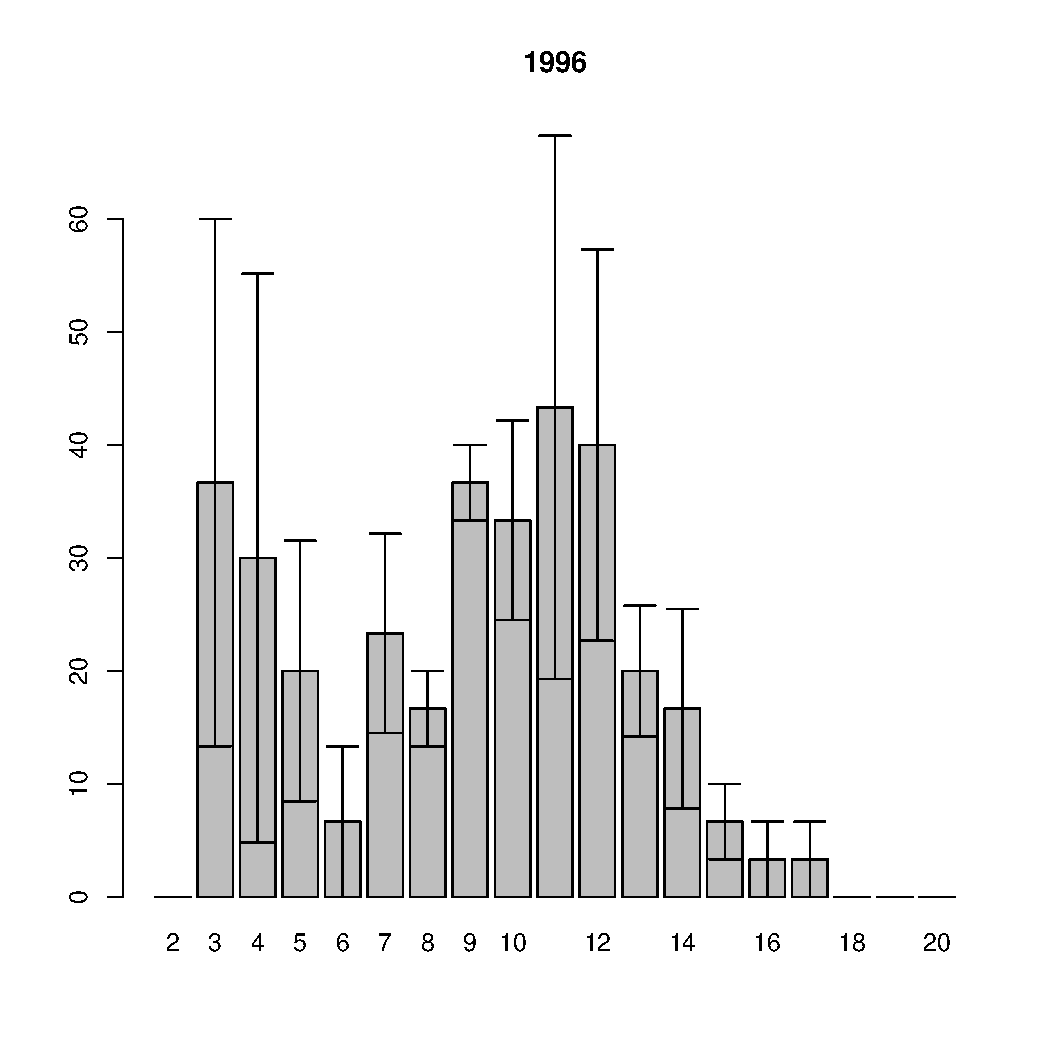
\includegraphics[width=14mm]{../White_Sea/Estuatiy_Luvenga/sizestr2_1996_.pdf}
\includegraphics[width=14mm]{../White_Sea/Estuatiy_Luvenga/sizestr2_1999_.pdf}
\includegraphics[width=14mm]{../White_Sea/Estuatiy_Luvenga/sizestr2_2002_.pdf}
\includegraphics[width=14mm]{../White_Sea/Estuatiy_Luvenga/sizestr2_2005_.pdf}
\includegraphics[width=14mm]{../White_Sea/Estuatiy_Luvenga/sizestr2_2008_.pdf}
\includegraphics[width=14mm]{../White_Sea/Estuatiy_Luvenga/sizestr2_2011_.pdf}
\end{figure}
\begin{figure}[h]
\includegraphics[width=14mm]{../White_Sea/Estuatiy_Luvenga/sizestr2_1994_.pdf}
\includegraphics[width=14mm]{../White_Sea/Estuatiy_Luvenga/sizestr2_1997_.pdf}
\includegraphics[width=14mm]{../White_Sea/Estuatiy_Luvenga/sizestr2_2000_.pdf}
\includegraphics[width=14mm]{../White_Sea/Estuatiy_Luvenga/sizestr2_2003_.pdf}
\includegraphics[width=14mm]{../White_Sea/Estuatiy_Luvenga/sizestr2_2006_.pdf}
\includegraphics[width=14mm]{../White_Sea/Estuatiy_Luvenga/sizestr2_2009_.pdf}
\includegraphics[width=14mm]{../White_Sea/Estuatiy_Luvenga/sizestr2_2012_.pdf}
\end{figure}
\end{frame}

\begin{frame}{Динамика размерной структуры {\it Macoma~balthica}}
%непонятно как забить в один-два-три слайда
Южная губа. Ежегодное пополнение.
\begin{figure}[h]
\includegraphics[width=20mm]{../White_Sea/Ryashkov_YuG/YuG_2001_.pdf}
\includegraphics[width=20mm]{../White_Sea/Ryashkov_YuG/YuG_2004_.pdf}
\includegraphics[width=20mm]{../White_Sea/Ryashkov_YuG/YuG_2007_.pdf}
\includegraphics[width=20mm]{../White_Sea/Ryashkov_YuG/YuG_2010_.pdf}
\end{figure}
\begin{figure}[h]
\includegraphics[width=20mm]{../White_Sea/Ryashkov_YuG/YuG_2002_.pdf}
\includegraphics[width=20mm]{../White_Sea/Ryashkov_YuG/YuG_2005_.pdf}
\includegraphics[width=20mm]{../White_Sea/Ryashkov_YuG/YuG_2008_.pdf}
\includegraphics[width=20mm]{../White_Sea/Ryashkov_YuG/YuG_2011_.pdf}
\end{figure}
\begin{figure}[h]
\includegraphics[width=20mm]{../White_Sea/Ryashkov_YuG/YuG_2003_.pdf}
\includegraphics[width=20mm]{../White_Sea/Ryashkov_YuG/YuG_2006_.pdf}
\includegraphics[width=20mm]{../White_Sea/Ryashkov_YuG/YuG_2009_.pdf}
\includegraphics[width=20mm]{../White_Sea/Ryashkov_YuG/YuG_2012_.pdf}
\end{figure}
\end{frame}

\begin{frame}{Динамика размерной структуры {\it Macoma~balthica}}
%непонятно как забить в один-два-три слайда

\begin{figure}[h]
\includegraphics[width=25mm]{../Barenc_Sea/Dalnezeleneckaya/DZ_2002_.pdf}
\includegraphics[width=25mm]{../Barenc_Sea/Dalnezeleneckaya/DZ_2004_.pdf}
\includegraphics[width=25mm]{../Barenc_Sea/Dalnezeleneckaya/DZ_2006_.pdf}
\includegraphics[width=25mm]{../Barenc_Sea/Dalnezeleneckaya/DZ_2008_.pdf}
\end{figure}
\begin{figure}[h]
\includegraphics[width=25mm]{../Barenc_Sea/Dalnezeleneckaya/DZ_2003_.pdf}
\includegraphics[width=25mm]{../Barenc_Sea/Dalnezeleneckaya/DZ_2005_.pdf}
\includegraphics[width=25mm]{../Barenc_Sea/Dalnezeleneckaya/DZ_2007_.pdf}
\begin{minipage}{25 mm}
Дальний пляж г.~Дальнезеленецкая
\end{minipage}
\end{figure}
\end{frame}


	\section{Динамика пополнения поселений маком}
\begin{frame}{Динамика численности годовалых особей {\it Macoma~balthica}}
% тут кроме динамики непонятно что? Корреляции с взрослыми. корреляции с половозрелыми. Корреляции с температурами.
\begin{figure}
\begin{minipage}[b]{.49\linewidth}
	\begin{center}
\tiny{Эстуарий р.~Лувеньги}
\includegraphics[width=49mm]{../White_Sea/Estuatiy_Luvenga/Estuary_N_oneyear.pdf}
	\end{center}
	\end{minipage}
\hfil %Это пружинка отодвигающая рисунки друг от друга
	\begin{minipage}[b]{.49\linewidth}
	\begin{center}
\tiny{ЗРС о.~Ряшкова}
\includegraphics[width=49mm]{../White_Sea/Ryashkov_ZRS/ZRS_N_oneyear.pdf}
	\end{center}
	\end{minipage}
\end{figure}
\end{frame}


\end{document}
